\chapter{Hardware Characterisation}
\label{chap:hardware}
\chaptoc{}

% ########################################

\newpage
\section{Introduction}
\label{sec:hardware_intro}
\begin{colsection}

In this chapter I detail my work characterising and modelling the GOTO hardware. This work was carried out predominantly in the first year and a half of my PhD, prior to GOTO's commissioning in 2017.
%
\begin{itemize}
    \item In \nref{sec:detectors} I describe and give the results of the in-lab detector characterisation tests I ran on the GOTO CCD cameras.
    \item In \nref{sec:throughput} I detail the throughput model of the GOTO optical system that I created.
    \item In \nref{sec:photometry} I apply the results of the previous two sections to predict the photometric properties of GOTO images, before comparing them to real observations taken once GOTO was fully operational.
\end{itemize}
%
All work described in this chapter is my own unless otherwise indicated, and has not been published elsewhere.

\end{colsection}

% ########################################

\newpage
\section{Detector properties}
\label{sec:detectors}
\begin{colsection}

% ~~~~~~~~~~~~~~~~~~~~

\begin{colsection}

CCD cameras have a variety of characteristic parameters advertised by the manufacturers, including sources of noise. As described in \aref{sec:goto_design}, GOTO uses MicroLine ML50100 CCD cameras manufactured by \glsfirst{fli}, which contain KAF-50100 CCD sensors manufactured by ON Semiconductor. Both manufactures produce specification sheets advertising expected parameters\footnote{ML50100 available at \url{http://www.flicamera.com/spec_sheets/ML50100.pdf}}\textsuperscript{,}\footnote{KAF-50100 available at \href{http://www.onsemi.com/pub/Collateral/KAF-50100-D.PDF}{\texttt{http://www.onsemi.com/pub/Collateral/KAF-50100-D.pdf}}}. Confirming these under laboratory conditions is important before the detectors are used to take scientific images on the telescope. FLI carried out a limited series of tests on the cameras before selling them, but carrying out our own tests ensures that our cameras meet the specifications, and also allows independent measurements of the key parameters.

\end{colsection}

% ~~~~~~~~~~~~~~~~~~~~
\subsection{Sources of CCD noise}
\label{sec:noise}
\begin{colsection}

There are many sources of noise in images taken with CCD cameras. The most important noise sources for astronomical images are \citep{CCDs}:
%
\begin{itemize}
    \item \emph{Shot noise} derived from counting photo-electrons from the source and background.
    \item \emph{Dark current noise} from thermally generated electrons within the sensor.
    \item \emph{Read-out noise} from the detector and CCD controller electronics.
    \item \emph{Fixed-pattern noise} from different sensitivities between pixels.
    \item \emph{Bias}, an offset in counts added to each pixel which can vary with time.
\end{itemize}

The shot noise ($\sigma_\text{N}$) arises as photons from the target object arrive at the sensor at irregular intervals. The photon arrival time is a Poisson distribution, and if the number of electrons counted is $N$ for large numbers it tends towards a Gaussian distribution with mean $N$ and standard deviation $\sigma_\text{N} = \sqrt{N}$. When taking on-sky astronomical observations there are two sources of shot noise, from the target object ($\sigma_\text{obj}$) and the background sky ($\sigma_\text{sky}$), but the latter is not relevant for the in-lab tests described in this section.

Dark current noise ($\sigma_\text{D}$) is due to electrons produced by thermal excitations, which are indistinguishable from photo-electrons and increase with exposure time. As this is also a photon counting measurement it follows a Poisson distribution, so the noise $\sigma_\text{DC} = \sqrt{D}$ where $D$ is the dark current per pixel. The dark current depends on temperature: cooling the cameras reduces the thermal excitations and therefore reduces the dark current.

Read-out noise ($\sigma_\text{RO}$) depends on the quality of the CCD outputs and readout electronics, and on the the speed data is read out from the CCD.\ The FLI MicroLine cameras read out at a fixed clock frequency of \SI{8}{\mega\hertz} per pixel, but other astronomical cameras have variable read-out speeds. Since read-out noise is a property of the output electronics, it is independent of signal or the exposure time used, and therefore it can be represented by a constant value for each frame, $\sigma_\text{RO} = R$, measured in electrons per pixel. The MicroLine cameras have two channels with independent readouts, so each will have an independent read-out noise.

Fixed-pattern noise ($\sigma_\text{FP}$, also called flat-field noise) is due to the small differences in size and response between pixels. It it increases linearly with the electron count, including source ($N$), background ($N_\text{sky}$) and dark ($D$) electrons (the fixed-pattern noise can be further broken down into the photo response non-uniformity and dark signal non-uniformity, but we will consider it as a single noise source). It can be parametrised as $\sigma_\text{FP} = k_\text{FP}(N+N_\text{sky}+D)$ where $k_\text{FP}$ is a dimensionless constant of proportionality describing the fixed-pattern noise as a fraction of the full-well capacity. Scientific CCD cameras typically have very small non-uniformities between pixels, so $k_\text{FP}$ is usually $<1\%$, but this noise source can dominate when the signal count is high. However as the fixed-pattern noise is linearly related to the number of counts recorded  it can easily be removed by flat fielding, so the contribution from the fixed-pattern noise is negligible in calibrated astronomical images.

Finally, the bias level is an offset in counts applied to each pixel independent of the input signal. A large bias level is applied each pixel by CCD manufacturers to prevent negative counts from being recorded due to fluctuations in the read-out noise. Across a frame the bias level will show structure due to being a different offset in each pixel, but it is simple to remove by subtracting a master bias frame. The bias level can change by a few counts during a night due to changes in the temperature. Bias should be measured regularly as any large changes might indicate a problem with the detector. The MicroLine cameras also include an overscan region (see \aref{sec:chip_layout}), which gives an independent measurement of the typical bias level for every image.

The noise sources described above (aside from the bias) are all independent Gaussian random variables, and therefore are added in quadrature to get the total noise per pixel

\begin{equation}
    \begin{split}
        \sigma_\text{Total}^2 & = \sigma_\text{obj}^2 +
                                  \sigma_\text{sky}^2 +
                                  \sigma_\text{DC}^2 +
                                  \sigma_\text{RO}^2 +
                                  \sigma_\text{FP}^2 \\
                              & = N + N_\text{sky} + D + R^2 + k_\text{FP}^2{(N+N_\text{sky}+D)}^2.
    \end{split}
    \label{eq:noise}
\end{equation}

\end{colsection}

% ~~~~~~~~~~~~~~~~~~~~
\subsection{In-lab tests}
\label{sec:camera_tests}
\begin{colsection}

The initial deployment of GOTO was delayed for several months, due to delays on-site at the observatory on La Palma and manufacturing the unit telescopes. The first set of four cameras however had already been purchased from FLI, and the delay gave time to test them in the lab in Sheffield in 2016. The second set of cameras were also purchased long before the second four unit telescopes were built; these were also brought to Sheffield  in 2018 so the same tests could be repeated. A list of the nine FLI cameras bought for GOTO is given in \aref{tab:cameras}. Each camera is given a name (Camera 1, Camera 2 etc.) based on the order of their serial numbers. These names are used throughout this section but do not necessarily match which GOTO unit telescope they were assigned to, and the cameras on La Palma are sometimes swapped around to allow for repairs.

\begin{table}[t]
    \begin{center}
        \begin{tabular}{c|ccc} %chktex 44
            Name     & Serial number & Set & Tested \\
            \midrule
            Camera 1 & ML0010316     &   1 & May---June 2016     \\
            Camera 2 & ML0330316     &   1 & March---May 2016    \\
            Camera 3 & ML0420516     &   1 & May---June 2016     \\
            Camera 4 & ML0430516     &   1 & May---June 2016     \\
            Camera 5 & ML5644917     &   2 & May---June 2018     \\
            Camera 6 & ML6054917     &   2 & May---June 2018     \\
            Camera 7 & ML6094917     &   2 & May---June 2018     \\
            Camera 8 & ML6304917     &   2 & May---June 2018     \\
            Camera 9 & ML6314917     &   2 & \textit{not tested} \\
        \end{tabular}
    \end{center}
    \caption[List of GOTO cameras]{
        A list of the 9 GOTO cameras, with assigned names, serial numbers and dates when the tests were carried out. The ninth camera (bought as a spare) was retained by Warwick for their own use, and was not tested in Sheffield.
    }\label{tab:cameras}
\end{table}

The characterisation tests consisted of taking a series of calibration frames with each camera. Three types of images were needed:

\begin{itemize}
    \item Zero-second dark exposures, to construct bias frames (see \aref{sec:bias}).
    \item Long (30 minute) dark exposures at different temperatures, to measure the dark current (see \aref{sec:dc}).
    \item Flat illuminated frames at different exposure times, to construct photon transfer curves to measure read-out noise, gain and fixed-pattern noise (see \aref{sec:ptc}), and to measure linearity (see \aref{sec:lin}).
\end{itemize}

The cameras were tested using two different test setups. \aref{fig:dark_photo} shows the setup for taking dark frames: the cameras are face down and covered by a sheet. The long dark exposures required were taken overnight to minimise the background light reaching the detectors. The flat fields were harder to take. A LCD monitor showing a dark screen was used, with sheets of paper between the camera and the monitor to reduce the illumination. This is shown in \aref{fig:flat_photo}.

\begin{figure}[p]
    \begin{center}
        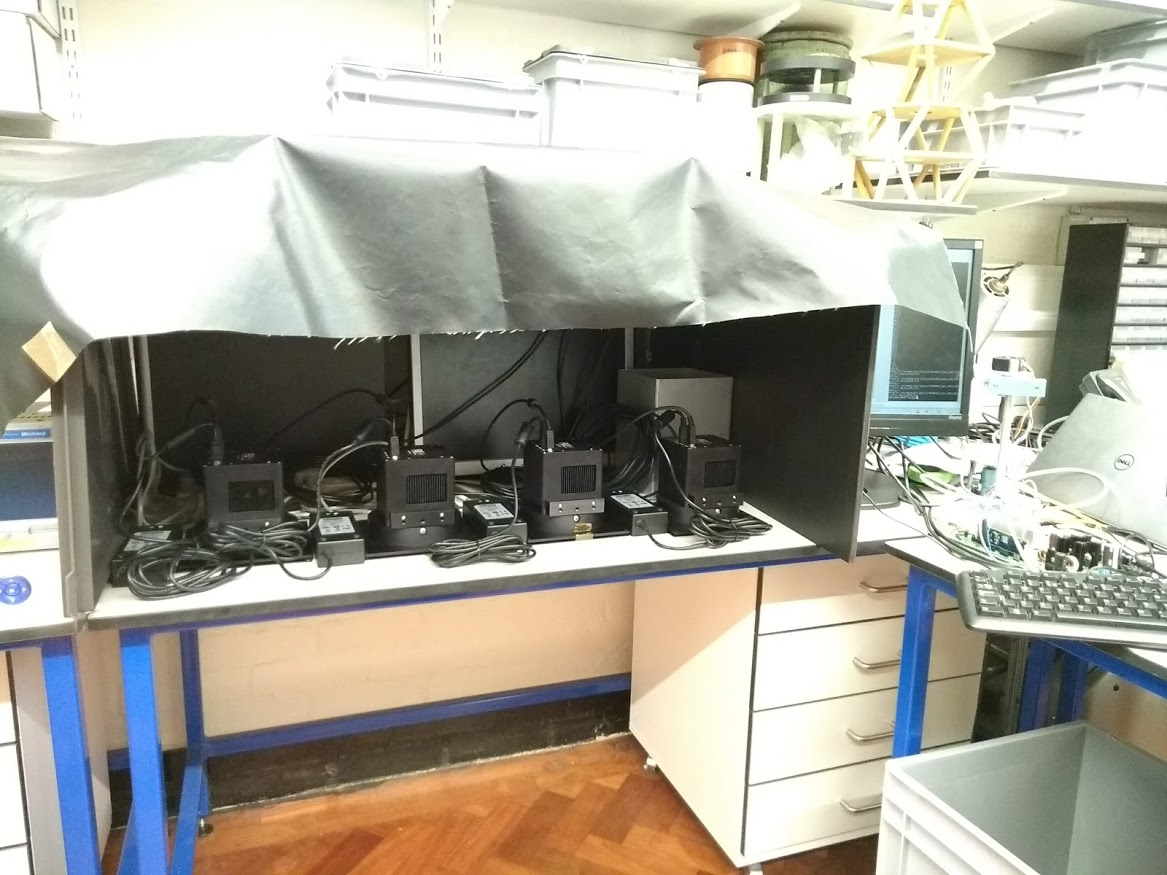
\includegraphics[width=0.75\textwidth]{images/dark_photo.jpg}
    \end{center}
    \caption[The dark frame test setup]{
        A photo of the dark frame test setup in the lab in Sheffield. Dark frames were taken at night with the cover down to minimise the ambient light.
    }\label{fig:dark_photo}
\end{figure}

\begin{figure}[p]
    \begin{center}
        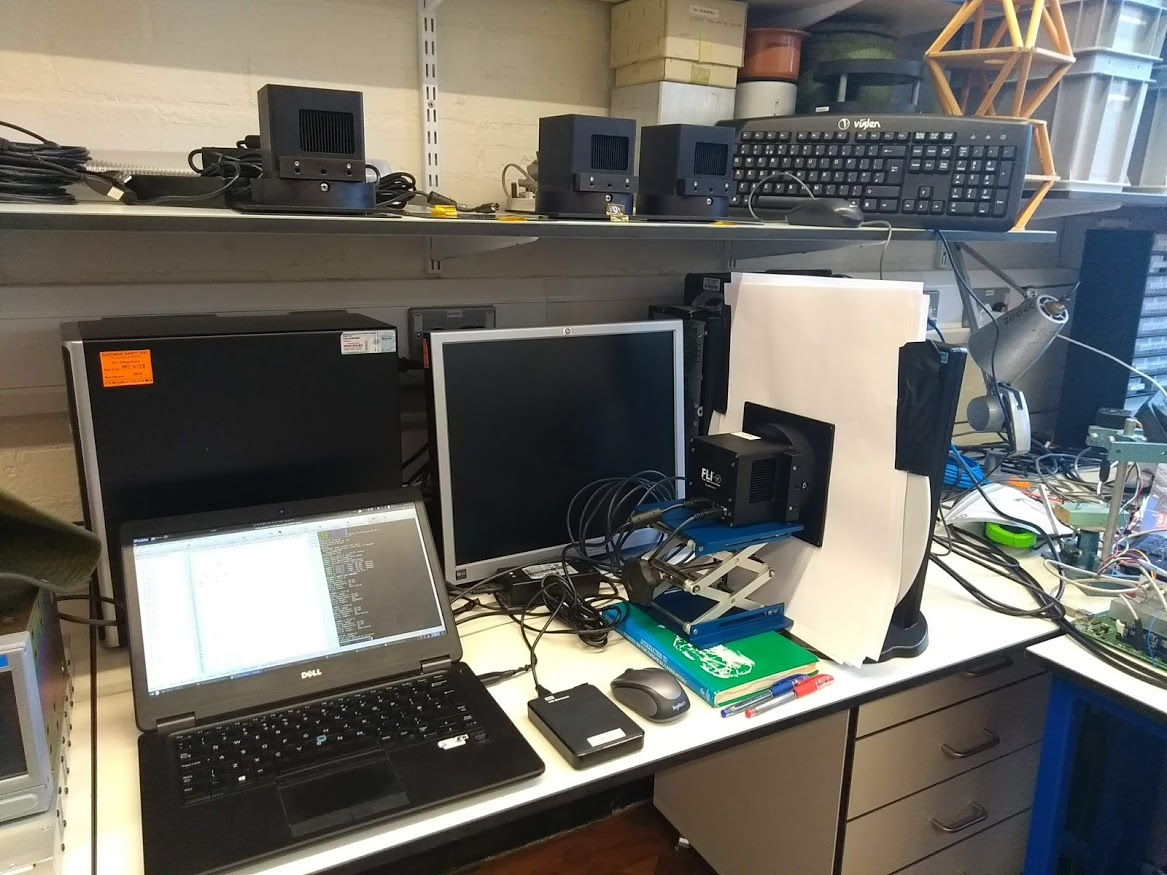
\includegraphics[width=0.75\textwidth]{images/flat_photo.jpg}
    \end{center}
    \caption[The flat field test setup]{
        A photo of the flat field test setup. A spare computer monitor was used as a flat screen, with sheets of paper placed in front of the camera to reduce the illumination. The cover shown in \aref{fig:dark_photo} was also placed over the setup.
    }\label{fig:flat_photo}
\end{figure}

\clearpage

\end{colsection}

% ~~~~~~~~~~~~~~~~~~~~
\newpage
\subsection{CCD sensors}
\label{sec:chip_layout}
\begin{colsection}

As mentioned previously, the MicroLine ML50100 cameras used by GOTO contain KAF-50100 \glsfirst{ccd} sensors manufactured for FLI by ON Semiconductor\footnote{\url{http://www.onsemi.com/}}. These are high-resolution, front-illuminated CCDs with two read-out channels. The detector includes a microlens array to focus light onto each pixel, as well as a multilayer anti-reflective coating. The \glsfirst{qe} curve for the detector is shown in \aref{fig:qe} in \aref{sec:qe}.

The sensor consists of a 50-megapixel CCD with $\SI{6}{\micro\metre} \times \SI{6}{\micro\metre}$ square pixels. The layout of the sensor is shown in \aref{fig:chip}, adapted from the ON Semiconductor sensor specification sheet. The sensor has $8304 \times 6220$ pixels with an imaging area of $8176 \times 6132$ pixels. When taking data in full-frame mode the camera outputs an $8304 \times 6220$ array. Surrounding the image area on each edge are 16 \emph{active buffer pixels}, which are light-sensitive but not considered part of the primary active region (they are not tested for deformities by the manufacturer). Around the edge of the active area is a border of light-shielded \emph{dark reference pixels}. These pixels do not respond to light and therefore can be used as a dark current reference. At the beginning and end of each row there is also a test column with 4 blank columns either side, as well as a test row at the end of each frame; these are used to test charge transfer efficiency during the manufacturing process. Finally, at the start of each row the register reads out a test pixel, used in the readout process, followed by 10 \emph{dummy pixels} which do not correspond to physical pixels on the sensor. These dummy pixels form an overscan region which can be used to measure the bias level.

A sample frame from Camera 2 is shown in \aref{fig:frame} at high contrast. The extra regions around the image area are visible, including the dark reference and overscan regions.

\begin{figure}[p]
    \begin{center}
        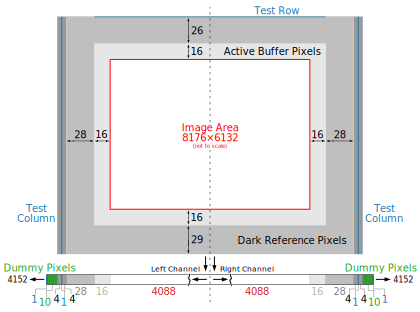
\includegraphics[width=0.85\textwidth]{images/chip}
    \end{center}
    \caption[The layout of the CCD chips in the MicroLine cameras used by GOTO]{
        The layout of the CCD chips in the MicroLine cameras used by GOTO.\@ The central image area is not shown to scale, but the surrounding rows and columns are all in proportion.
    }\label{fig:chip}
\end{figure}

\begin{figure}[p]
    \begin{center}
        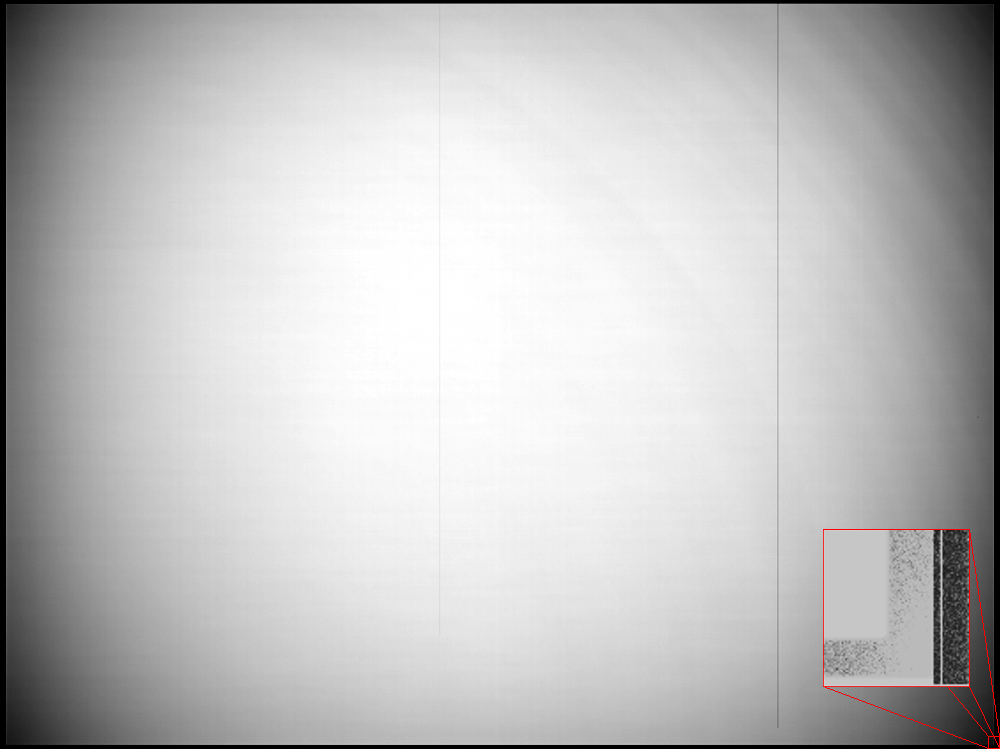
\includegraphics[width=0.65\textwidth]{images/sample.png}
    \end{center}
    \caption[A sample bright frame from one of the MicroLine cameras]{
        A sample bright frame from one of the MicroLine cameras. The highlighted area in the corner shows some of the features described in \aref{fig:chip}.
    }\label{fig:frame}
\end{figure}

\clearpage

\end{colsection}

% ~~~~~~~~~~~~~~~~~~~~
\newpage
\subsection{Bias}
\label{sec:bias}
\begin{colsection}

The bias level in each pixel can be measured by taking a dark, zero-second exposure image. This image will not include any electrons from a source or background, so the shot noise is zero, and as the dark current is proportional to the exposure time this will also be minimised (there will be a small component due to the time taken to read out the sensor). To account for the read-out noise multiple images are taken, 50 for each of the eight cameras, and combined to form a master bias frame by taking the median value in each pixel (to eliminate cosmic rays).

\aref{tab:bias} gives the median bias level from each master bias, measured within a 2000$\times$2000 pixel region in the centre of both channels, along with the standard deviation in the same region. The measured bias levels are all around 1000 counts, which would be typical for a bias level set by the manufacturer. Combining $N$ frames should reduce the noise by $\sqrt{N}$, and, as expected, the errors are equivalent to the read-out noise values given in \aref{tab:ptc} when converted into counts and reduced by a factor of $\sqrt{50}$ ($\approx 7$).

\begin{table}[t]
    \begin{center}
        \begin{tabular}{c|rr} %chktex 44
             & \multicolumn{2}{c}{Bias} \\
             & \multicolumn{2}{c}{(ADU)} \\
             & \multicolumn{1}{c}{L} & \multicolumn{1}{c}{R} \\
            \midrule
            Camera 1 & $971\pm3.6$ & $969\pm3.7$ \\
            Camera 2 & $989\pm3.3$ & $983\pm3.3$ \\
            Camera 3 & $1004\pm3.2$ & $991\pm3.1$ \\
            Camera 4 & $974\pm3.4$ & $1008\pm3.8$ \\
        \end{tabular}
        \hspace{0.5cm}
        \begin{tabular}{c|rr} %chktex 44
             & \multicolumn{2}{c}{Bias} \\
             & \multicolumn{2}{c}{(ADU)} \\
             & \multicolumn{1}{c}{L} & \multicolumn{1}{c}{R} \\
            \midrule
            Camera 5 & $994\pm2.9$ & $986\pm3.0$ \\
            Camera 6 & $984\pm2.7$ & $991\pm3.0$ \\
            Camera 7 & $992\pm3.1$ & $981\pm3.0$ \\
            Camera 8 & $1008\pm3.3$ & $1012\pm2.9$ \\
        \end{tabular}
    \end{center}
    \caption[Bias values]{
        Bias values for each camera.
    }\label{tab:bias}
\end{table}

\end{colsection}

% ~~~~~~~~~~~~~~~~~~~~
\subsection{Gain, read-out noise and fixed-pattern noise}
\label{sec:ptc}
\begin{colsection}

The gain, read-out and fixed-pattern noise of a CCD camera can be measured using the \glsfirst{ptc} method \citep{CCDs, PTC}. A photon transfer curve is a log-log plot of a signal value against the noise in the signal. To construct a photon transfer curve a series of bright exposures of a flat light source were taken with varying exposure times. For these images there is no background signal, the cameras were cooled meaning dark current noise is negligible (see \aref{sec:dc}), and the master bias frames created in \aref{sec:bias} were subtracted from each frame. The total noise per pixel in electrons is therefore given by \aref{eq:noise} as
%
\begin{equation}
    \sigma_\text{Total}^2 = N + R^2 + k_\text{FP}^2{(N)}^2.
    \label{eq:noise_2}
\end{equation}

The signal and total noise in \aref{eq:noise} are all in electrons (\elec), however the output of the camera's \glsfirst{adc} is a digital signal, $S$, measured in counts or \glsfirst{adu}. This signal is linearly related to the actual number of electrons detected $N$ through the gain $g$, in \elec/ADU, as
%
\begin{equation}
    N = g S.
    \label{eq:gain}
\end{equation}
%
The gain is an important parameter of a CCD, and is set by the manufacturer based on the properties of the detector. For example, if a CCD has the gain set to 3 \elec/ADU then pixels containing 0, 1 or 2 electrons would all have a measured value of 0 ADU;\@ this is a form of rounding error called quantisation error. If the camera had a read-out noise of 1 \elec{} per pixel then the readout-noise would be under-sampled, and setting a lower gain would be required. However, setting the gain too low results in the full-well capacity of each pixel being underutilised. The KAF-50100 detectors have a full well capacity of 40,300 electrons, and the cameras have a 16-bit ADC (meaning the signal from each pixel can vary from 0 to 65535 ($2^{16}-1$) ADU). If the gain is set to $0.5$ \elec/ADU then the ADC would saturate after reading 32,768 electrons, which is much less than the capacity of each pixel. Setting the gain therefore is a balance between these two effects.

As electrons and counts are proportional the noise in both is also proportional (i.e.\ as $N=gS$ from \aref{eq:gain},  $\sigma_\text{Total} = g\sigma_S$). Using these relationships \aref{eq:noise_2} can be converted to give the noise in ADU,
%
\begin{equation}
    \sigma_S^2 = \frac{1}{g} S + \frac{R^2}{g^2} + k_\text{FP}^2 S^2.
    \label{eq:ptc}
\end{equation}
%
This is a quadratic equation which relates the measured total signal $S$ to the variance in the signal $\sigma_S^2$, and can be fitted to a photon transfer curve to determine values for the gain $g$ (in \elec/ADU), read-out noise $R$ (still in \elec{}) and fixed-pattern noise $k_\text{FP}$ (dimensionless).

\begin{figure}[t]
    \begin{center}
        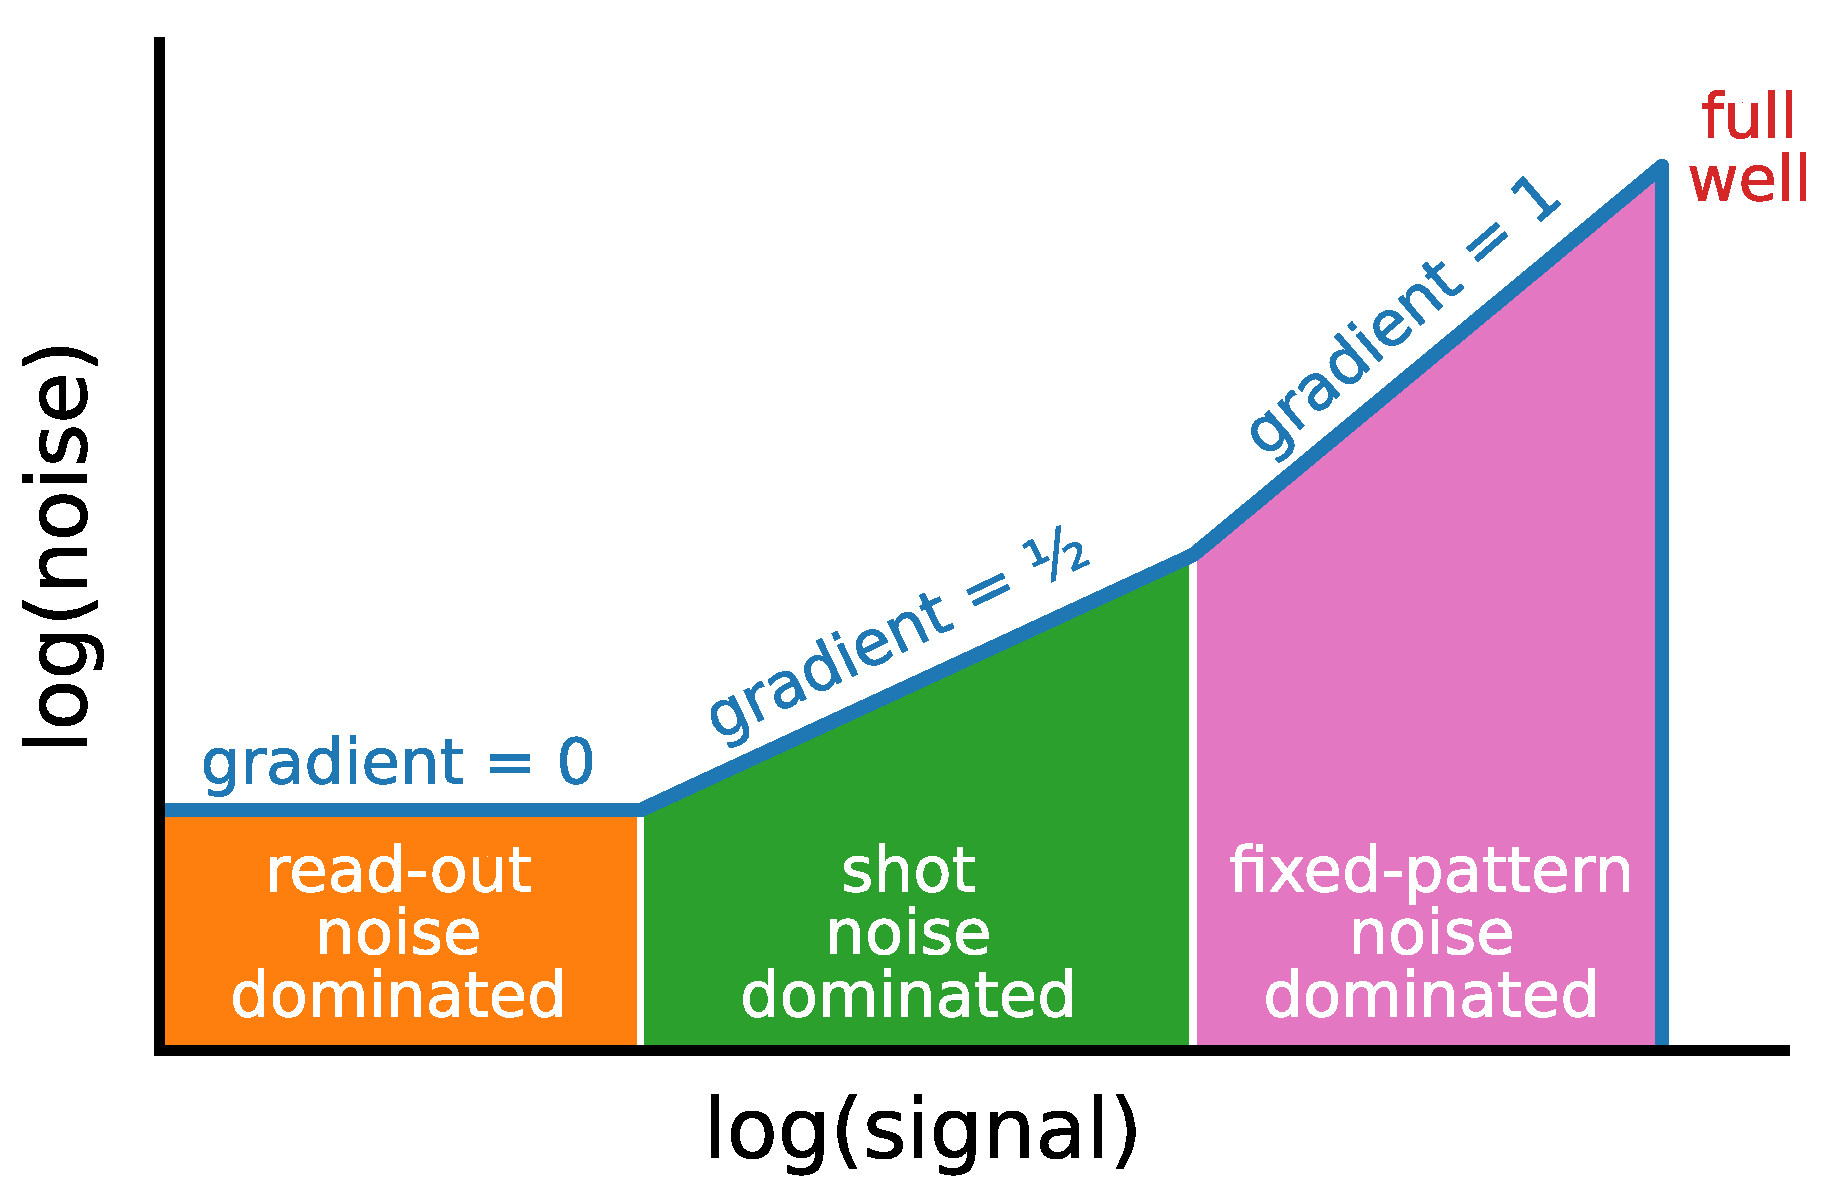
\includegraphics[width=0.8\textwidth]{images/ptc.pdf}
    \end{center}
    \caption[Key features of the photon transfer curve]{
        The key features of a photon transfer curve, adapted from \citet{CCDs}.
    }\label{fig:ptc_cartoon}
\end{figure}

The key features of a photon transfer curve are common for all CCDs, and are shown in cartoon form in \aref{fig:ptc_cartoon}. The first noise regime is when the signal is small: from \aref{eq:ptc} for small $S$ the noise is constant and equal to $R^2/g^2$, or the read-out noise in ADU.\@ At higher signals the noise is dominated by the shot noise which is proportional to $\sqrt{S}$, so this region has a gradient of 1/2 when plotted on the log-log axis. As the signal increases further the fixed-pattern noise begins to dominate, and, as this noise is proportional to the signal, this produces a gradient of 1 in the PTC.\@ Finally, the pixel reaches its full well capacity (assuming the gain has been set so this occurs before the ADU saturates), so the noise drops to zero.

\begin{table}[t]
    \begin{center}
        \begin{tabular}{l|cc|cc|cc|cc} %chktex 44
             &
            \multicolumn{2}{c|}{Gain} &
            \multicolumn{2}{c|}{RO noise} &
            \multicolumn{2}{c|}{FP noise} &
            \multicolumn{2}{c}{Saturation level} \\
            &
            \multicolumn{2}{c|}{(\elec/ADU)} &
            \multicolumn{2}{c|}{(\elec)} &
            \multicolumn{2}{c|}{(\%)} &
            \multicolumn{2}{c}{(ADU)} \\
             & L & R & L & R & L & R & L & R \\
            \midrule
            Camera 1 & 0.53 & 0.53 & 12.4 & 12.0 & 0.46 & 0.45 & 64568 & 64585 \\
            Camera 2 & 0.53 & 0.53 & 11.9 & 11.7 & 0.44 & 0.46 & 64552 & 64555 \\
            Camera 3 & 0.57 & 0.57 & 12.6 & 11.8 & 0.45 & 0.42 & 64540 & 64552 \\
            Camera 4 & 0.57 & 0.58 & 13.4 & 14.0 & 0.41 & 0.43 & 64577 & 64536 \\
            Camera 5 & 0.62 & 0.63 & 12.3 & 12.8 & 0.40 & 0.40 & 64544 & 64550 \\
            Camera 6 & 0.63 & 0.62 & 11.8 & 12.6 & 0.40 & 0.40 & 64554 & 64545 \\
            Camera 7 & 0.62 & 0.62 & 13.1 & 12.5 & 0.41 & 0.39 & 64544 & 64552 \\
            Camera 8 & 0.62 & 0.62 & 14.3 & 12.2 & 0.41 & 0.39 & 64529 & 64522 \
        \end{tabular}
    \end{center}
    \caption[Gain, read-out noise, fixed-pattern noise and saturation values]{
        Gain, read-out noise, fixed-pattern noise and saturation values found by fitting photon transfer curves for each camera.
    }\label{tab:ptc}
\end{table}

Photon transfer curves were constructed for all eight cameras, by taking flat fields of varying exposure times between \SI{0.01}{\second} and \SI{90}{\second}. Twelve 50$\times$50 pixel regions were selected across the field, and the mean and standard deviation of the pixel values within each region were plotted to form the PTC for each camera, shown in \aref{fig:ptcs}. \aref{eq:ptc} was then fitted to the data, and the resulting values for the gain ($g$), read-out noise ($R$) and fixed-pattern noise ($k_\text{FP}$) parameters are given in \aref{tab:ptc}. The saturation level for each channel was also measured as the maximum signal (the point where the PTC turns over and the noise drops), these values are also given in \aref{tab:ptc}.

The gain values are all around 0.6 \elec/ADU, and would have been set as such to maximise the dynamic range based on the full well capacity. The saturation levels are all around 64550, and 64550 $\times$ 0.6 $\approx$ 39,000 \elec, which matches the advertised 40,300 capacity. The read-out noise values also match the FLI specifications, which advertise a typical read-out noise of 12 \elec{} for the MicroLine cameras. Finally, the fixed-pattern noise is a low fraction of the signal ($<0.5\%$). This was to be expected, as modern CCD sensors have very low pixel non-uniformities.

\begin{figure}[p]
    \begin{center}
        \begin{minipage}[t]{0.49\textwidth}\vspace{10pt}
            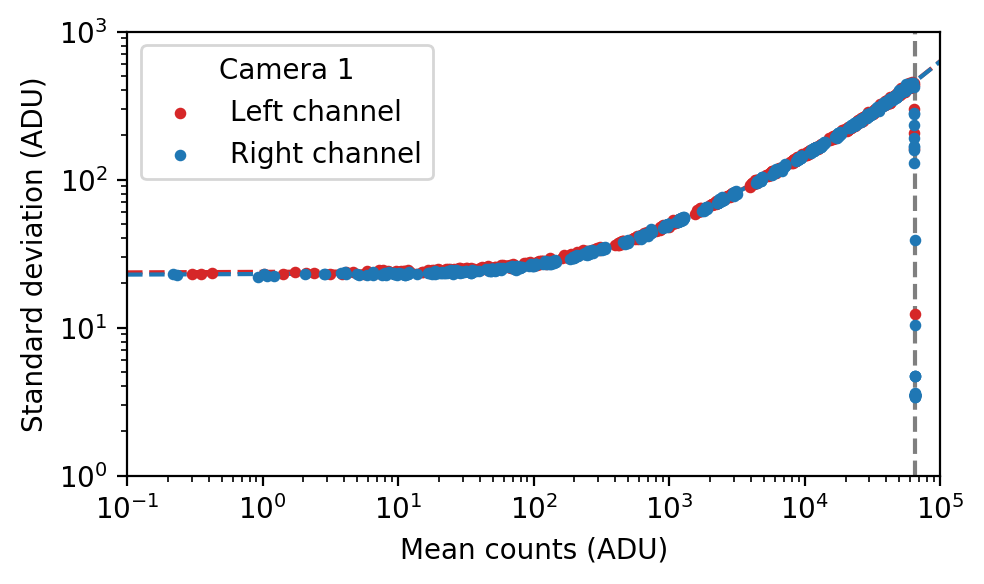
\includegraphics[width=\linewidth]{images/detectors/ptc_1.png}
        \end{minipage}
        \begin{minipage}[t]{0.49\textwidth}\vspace{10pt}
            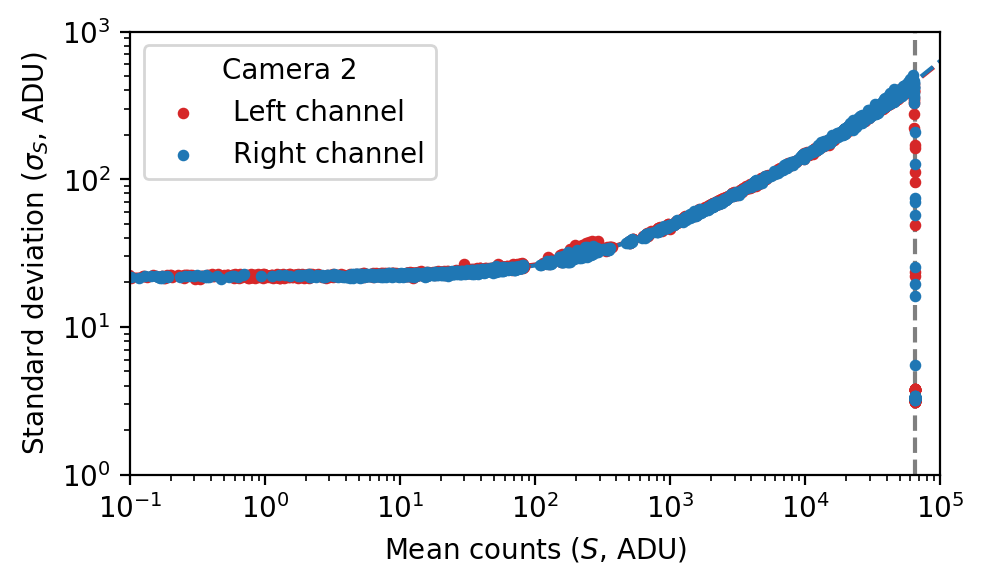
\includegraphics[width=\linewidth]{images/detectors/ptc_2.png}
        \end{minipage}

        \begin{minipage}[t]{0.49\textwidth}\vspace{10pt}
            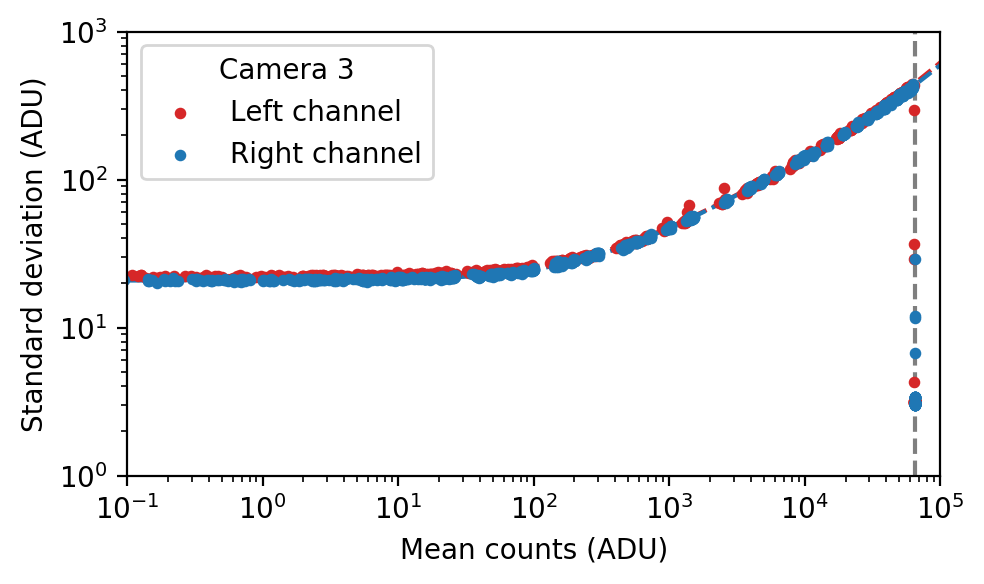
\includegraphics[width=\linewidth]{images/detectors/ptc_3.png}
        \end{minipage}
        \begin{minipage}[t]{0.49\textwidth}\vspace{10pt}
            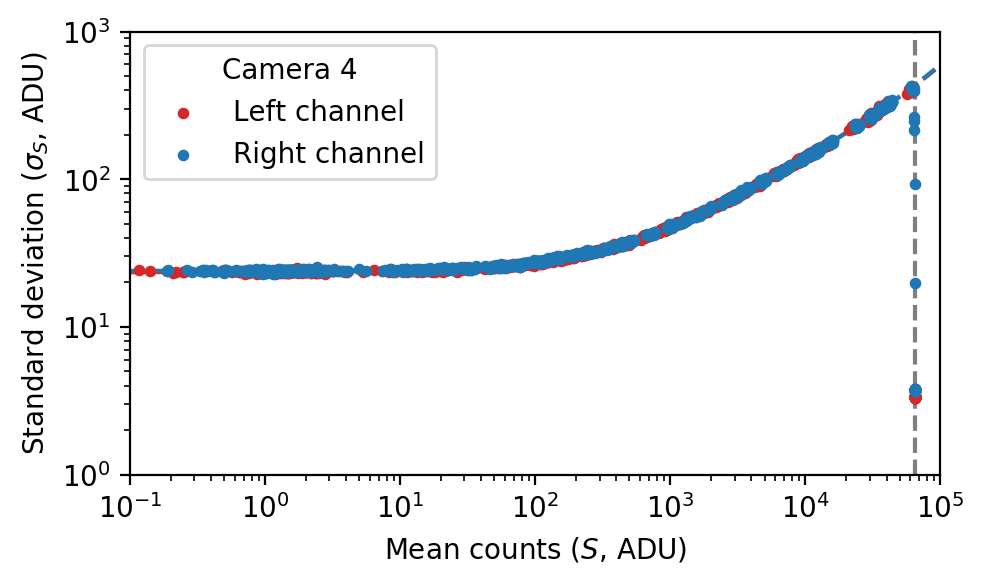
\includegraphics[width=\linewidth]{images/detectors/ptc_4.png}
        \end{minipage}

        \begin{minipage}[t]{0.49\textwidth}\vspace{10pt}
            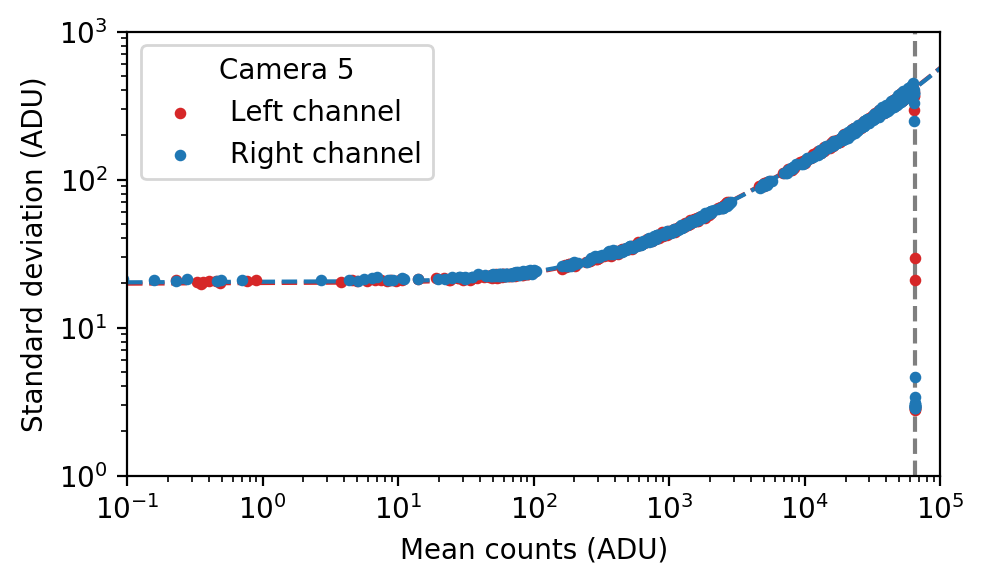
\includegraphics[width=\linewidth]{images/detectors/ptc_5.png}
        \end{minipage}
        \begin{minipage}[t]{0.49\textwidth}\vspace{10pt}
            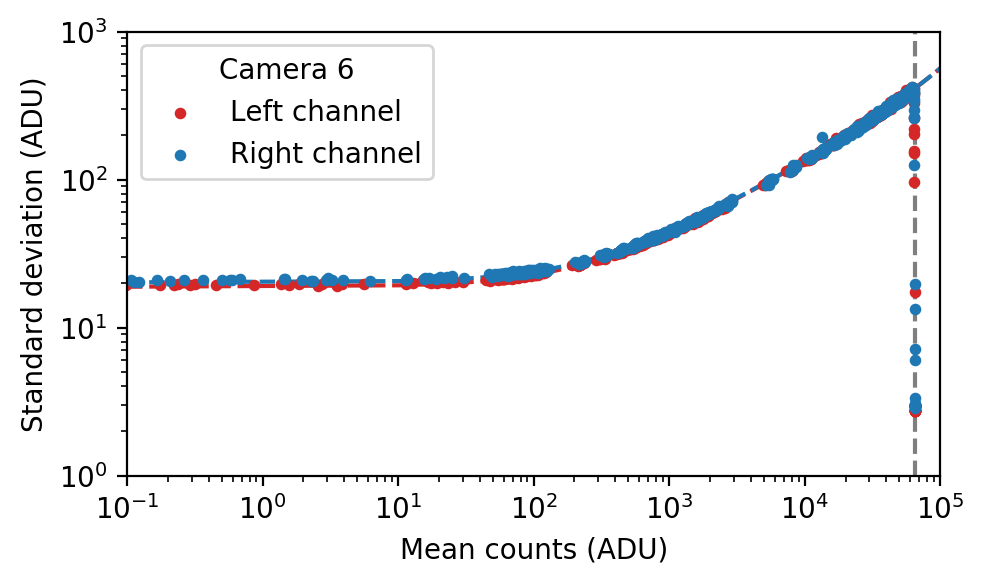
\includegraphics[width=\linewidth]{images/detectors/ptc_6.png}
        \end{minipage}

        \begin{minipage}[t]{0.49\textwidth}\vspace{10pt}
            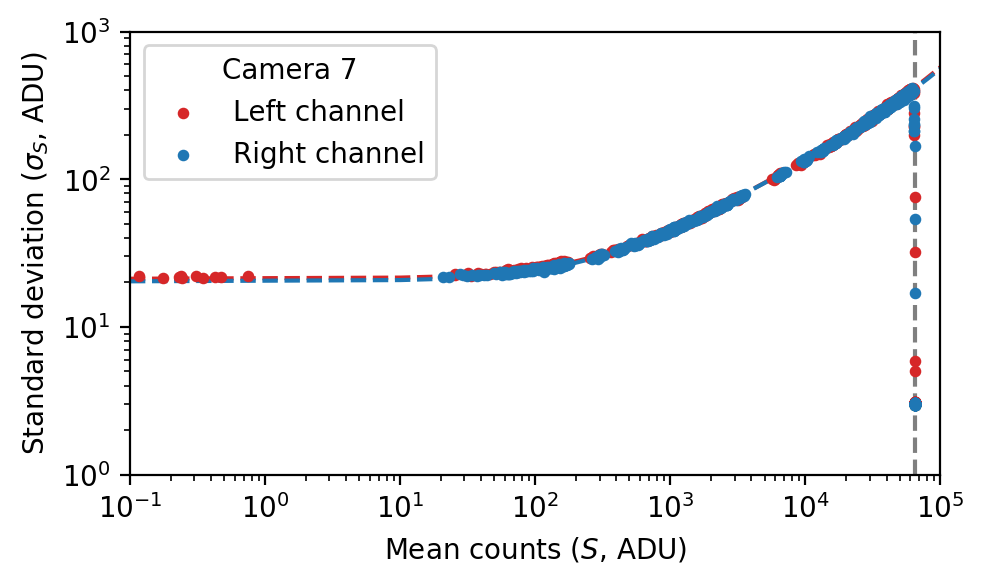
\includegraphics[width=\linewidth]{images/detectors/ptc_7.png}
        \end{minipage}
        \begin{minipage}[t]{0.49\textwidth}\vspace{10pt}
            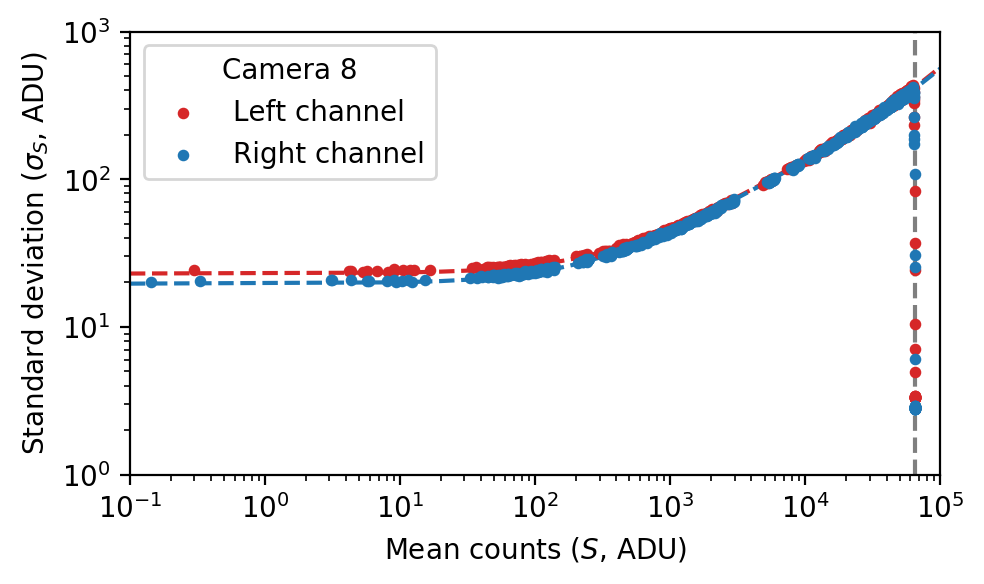
\includegraphics[width=\linewidth]{images/detectors/ptc_8.png}
        \end{minipage}
    \end{center}
    \caption[Photon transfer curve plots]{
        Photon transfer curve plots for each camera. The vertical dashed line shows the measured saturation level.
    }\label{fig:ptcs}
\end{figure}

\clearpage

\end{colsection}

% ~~~~~~~~~~~~~~~~~~~~
\newpage
\subsection{Dark current}
\label{sec:dc}
\begin{colsection}

Dark current noise is independent of the incoming signal but depends on the exposure time of the image. It also increases as a function of temperature, $T$. The dark current per second, $D$, increases at an exponential rate and can be modelled using the equation
%
\begin{equation}
    D(T) = Ae^{kT + C},
    \label{eq:dark_model}
\end{equation}
%
where $A$, $k$ and $C$ are constants. Dark current is usually defined as doubling after a fixed increase in temperature called the doubling temperature, $T_d$, so that if the dark current $D(T_0) = D_0$ then $D(T_0 + T_d) = 2D_0$. Redefining \aref{eq:dark_model} using these constants gives the equation for dark currant as
%
\begin{equation}
    D(T) = D_0 e^{\frac{\ln2}{T_d}(T + T_0)}.
    \label{eq:dc}
\end{equation}
%
The choice of $T_0$ is arbitrary, and is usually decided as a reasonable operating temperature by the CCD manufacturer. The FLI specifications give a value for the typical dark current at \SI{-25}{\celsius}, so that is the value of $T_0$ used in this test.

In order to find values for the dark current $D_0$ and doubling temperature $T_d$, a series of long (30 minute) dark exposures were taken with each camera at varying temperatures. The MicroLine cameras have an in-built air-cooled peltier cooler which can reach \SI{40}{\celsius} below the ambient temperature. The laboratory the tests were carried out were air-conditioned, but only to a typical office level and the cameras were unable to reach below \SI{-26}{\celsius} even when taking images in the middle of the night. The median dark signal was then measured in a 2000$\times$2000 pixel region in the centre of each channel, and divided by 1800 to get the dark current in ADU/second. This value was plotted against temperature, as shown in \aref{fig:dcs}. The points were fitted by \aref{eq:dc}, and the resulting values for the dark current and doubling temperature are given in \aref{tab:dc}.

\begin{table}[t]
    \begin{center}
        \begin{tabular}{c|cc|cc|rr} %chktex 44
             &
            \multicolumn{4}{c|}{Dark current per pixel} &
            \multicolumn{2}{c}{Doubling} \\
             &
            \multicolumn{4}{c|}{at \SI{-25}{\celsius}} &
            \multicolumn{2}{c}{temperature} \\
             &
            \multicolumn{2}{c|}{(ADU/s)} &
            \multicolumn{2}{c|}{(e-/s)} &
            \multicolumn{2}{c}{(\SI{}{\celsius})} \\
             & L & R & L & R &
             \multicolumn{1}{c}{L} & \multicolumn{1}{c}{R} \\
            \midrule
            Camera 1 & 0.0022 & 0.0017 & 0.0012 & 0.0009 &  7.9 &  6.7 \\
            Camera 2 & 0.0030 & 0.0027 & 0.0016 & 0.0014 &  8.9 &  8.2 \\
            Camera 3 & 0.0034 & 0.0036 & 0.0019 & 0.0020 & 10.7 & 10.9 \\
            Camera 4 & 0.0026 & 0.0030 & 0.0015 & 0.0017 &  9.5 & 10.2 \\
            Camera 5 & 0.0015 & 0.0017 & 0.0009 & 0.0011 &  6.6 &  7.2 \\
            Camera 6 & 0.0020 & 0.0017 & 0.0013 & 0.0011 &  7.5 &  6.8 \\
            Camera 7 & 0.0017 & 0.0014 & 0.0011 & 0.0008 &  7.6 &  6.5 \\
            Camera 8 & 0.0019 & 0.0015 & 0.0012 & 0.0009 &  7.5 &  6.5 \\
        \end{tabular}
    \end{center}
    \caption[Dark current values]{
        Dark current values for each camera. The conversion from ADU/s to \elec/s used the gain values given in \aref{tab:ptc}.
    }\label{tab:dc}
\end{table}

The FLI specification for dark current changed between the two test periods; initially the company gave a typical per-pixel value of 0.002~\elec/s at \SI{-25}{\celsius}, for the second set of cameras this was increased to 0.008~\elec/s. All the cameras were found to have a dark current well within the revised specification value, and all except Camera 3 are comfortably below the original 0.002~\elec/s specification.

The KAF-50100 specification includes a value for the doubling temperature of \SI{5.7}{\celsius} but the measured values are all higher than this. In practice the temperature dependence of the dark current is not important, the GOTO cameras are cooled to \SI{-20}{\celsius} in the evening and remain there through the night (\SI{-20}{\celsius} is used instead of \SI{-25}{\celsius} as during the summer on La Palma the ambient nightly temperature can reach higher than \SI{15}{\celsius}).

The dark current was also examined as a function of time since power on, as in some cameras there are a noticeable amount of free electrons left trapped in the lattice which take time to dissipate \citep{Liam}. No such trend was visible using the FLI cameras. Since the MicroLine cameras have the detector and cooler integrated into the same body there has to be some time spent waiting after power on for the camera to cool to the target temperature before any images can be taken, thus negating the effect.

\begin{figure}[p]
    \begin{center}
        \begin{minipage}[t]{0.49\textwidth}\vspace{10pt}
            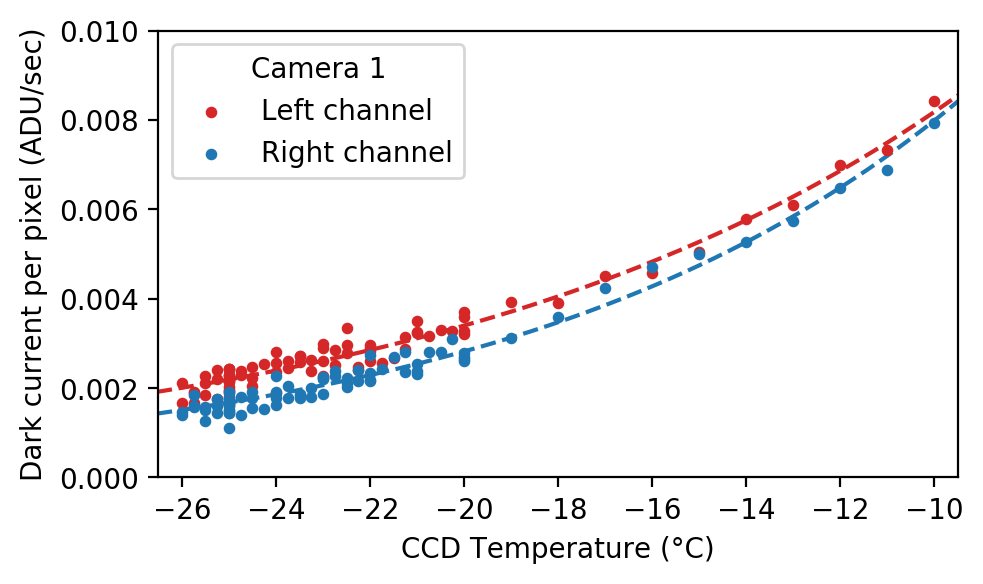
\includegraphics[width=\linewidth]{images/detectors/dc_1.png}
        \end{minipage}
        \begin{minipage}[t]{0.49\textwidth}\vspace{10pt}
            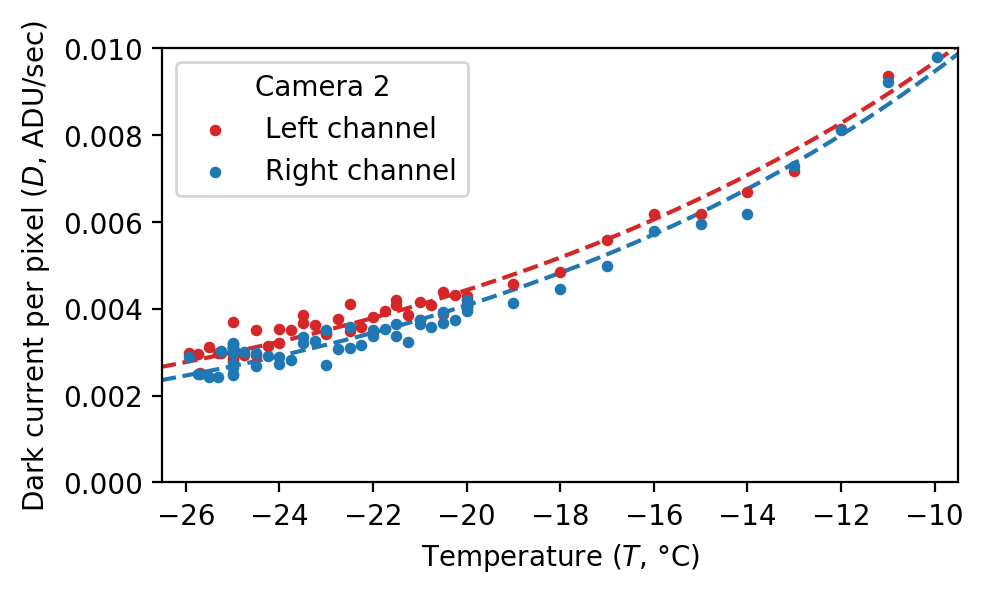
\includegraphics[width=\linewidth]{images/detectors/dc_2.png}
        \end{minipage}

        \begin{minipage}[t]{0.49\textwidth}\vspace{10pt}
            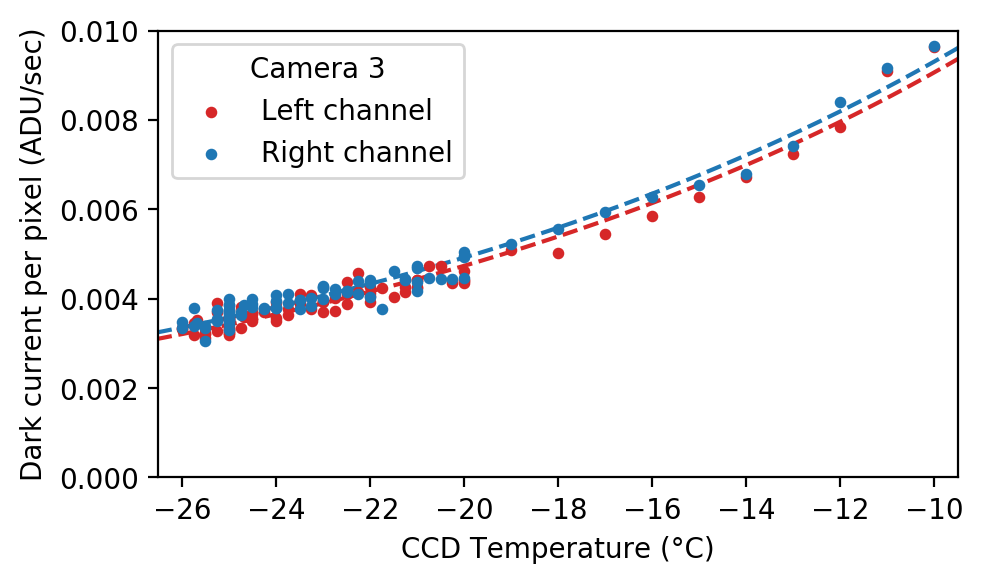
\includegraphics[width=\linewidth]{images/detectors/dc_3.png}
        \end{minipage}
        \begin{minipage}[t]{0.49\textwidth}\vspace{10pt}
            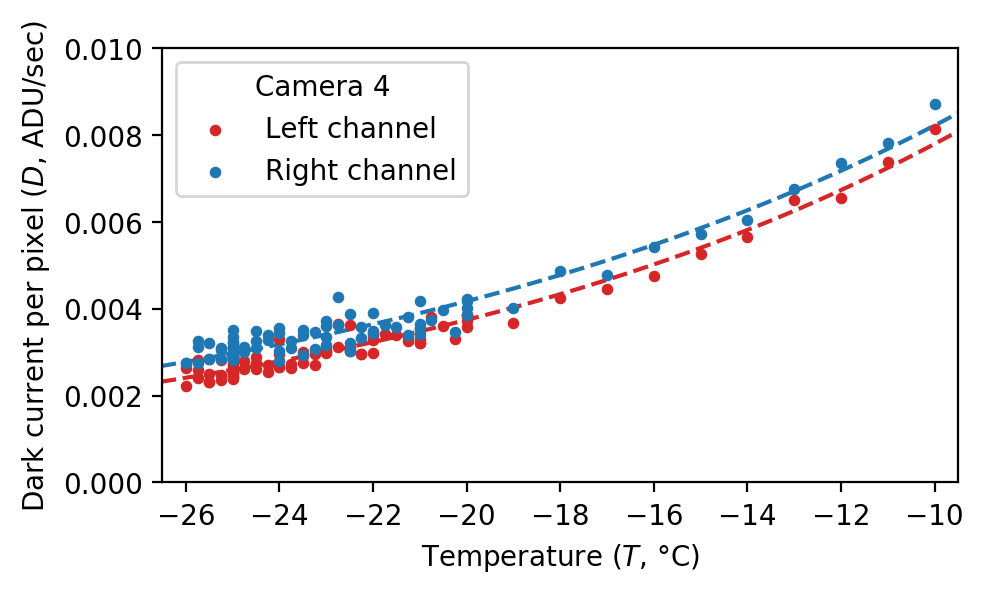
\includegraphics[width=\linewidth]{images/detectors/dc_4.png}
        \end{minipage}

        \begin{minipage}[t]{0.49\textwidth}\vspace{10pt}
            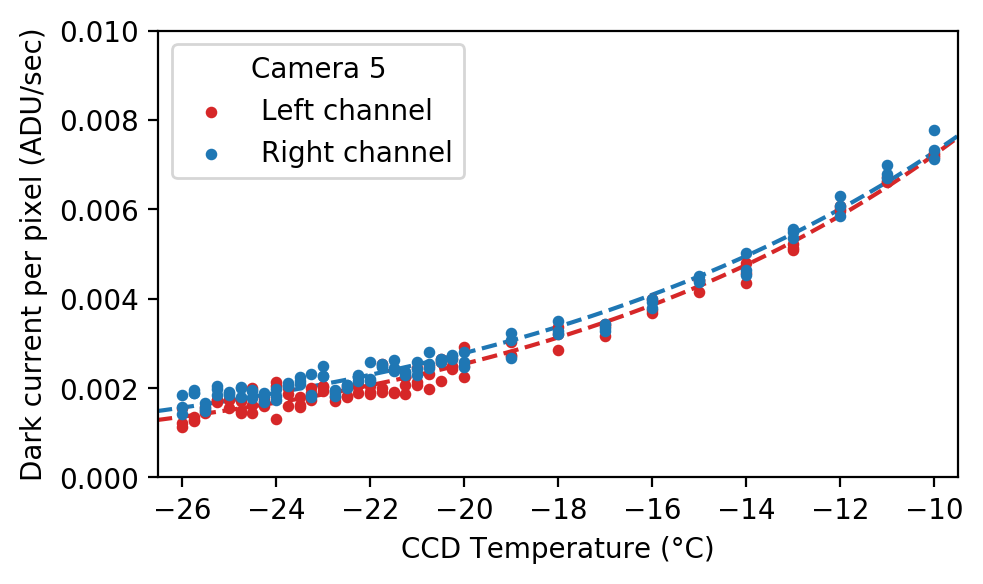
\includegraphics[width=\linewidth]{images/detectors/dc_5.png}
        \end{minipage}
        \begin{minipage}[t]{0.49\textwidth}\vspace{10pt}
            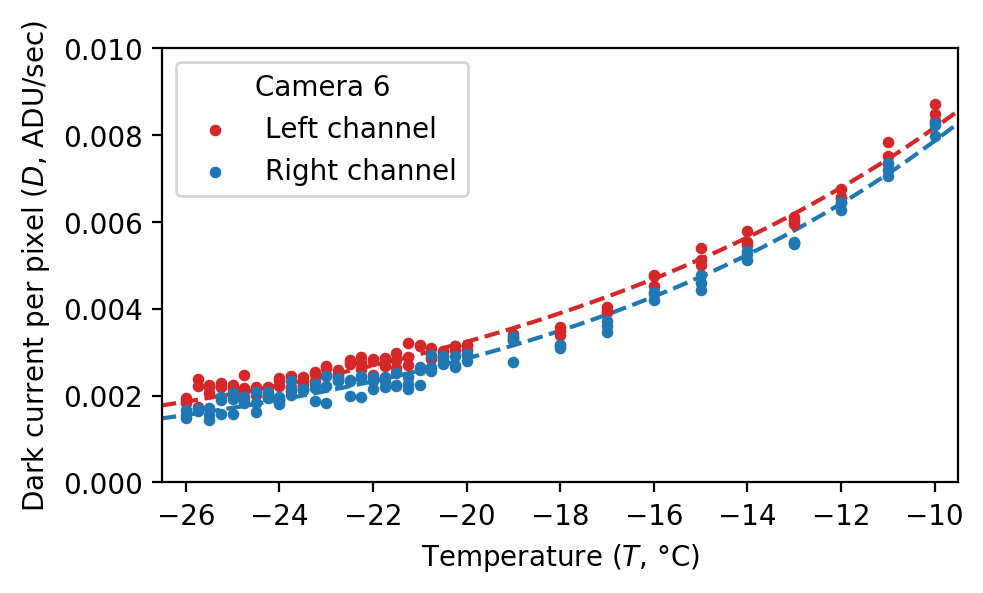
\includegraphics[width=\linewidth]{images/detectors/dc_6.png}
        \end{minipage}

        \begin{minipage}[t]{0.49\textwidth}\vspace{10pt}
            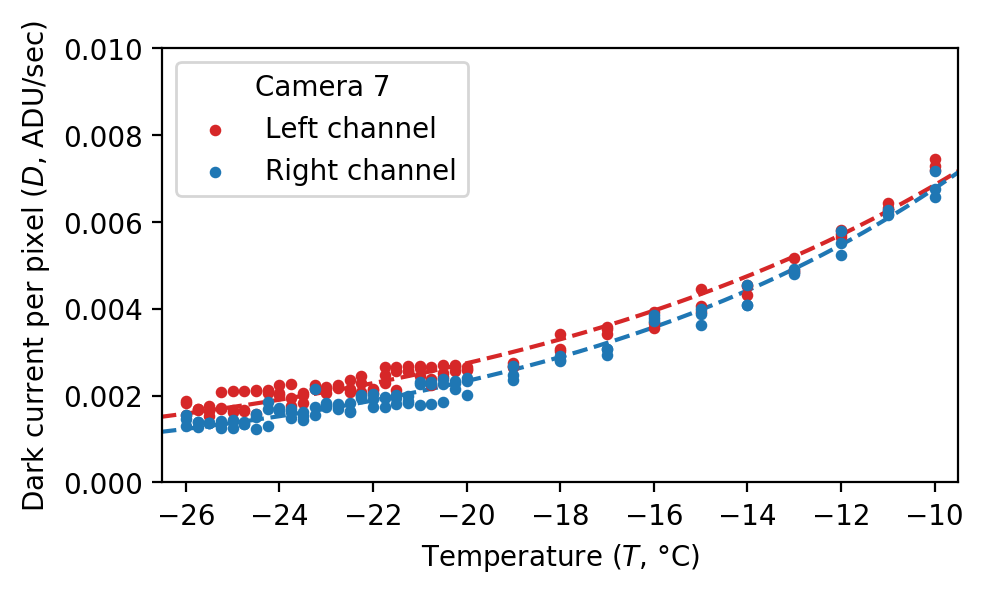
\includegraphics[width=\linewidth]{images/detectors/dc_7.png}
        \end{minipage}
        \begin{minipage}[t]{0.49\textwidth}\vspace{10pt}
            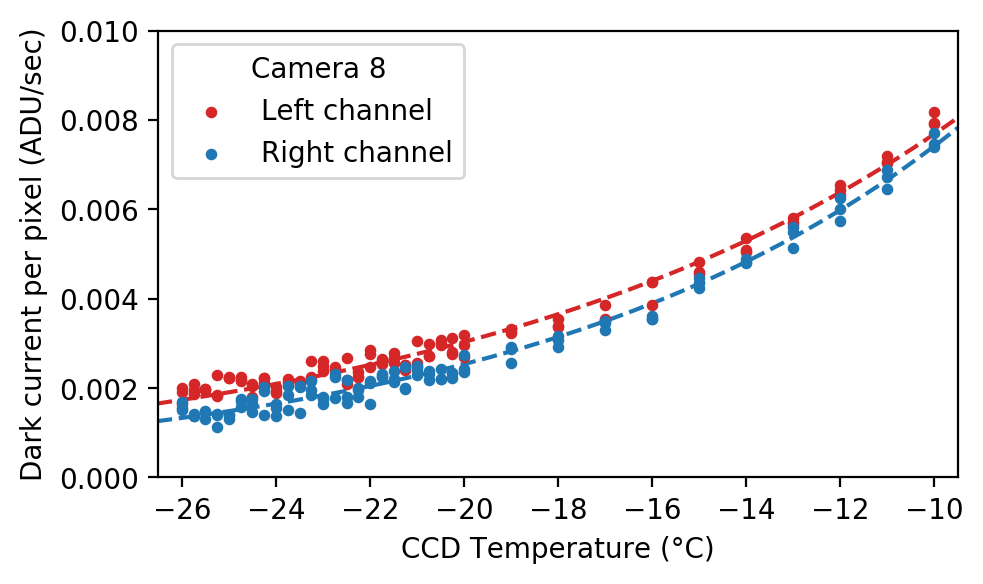
\includegraphics[width=\linewidth]{images/detectors/dc_8.png}
        \end{minipage}
    \end{center}
    \caption[Dark current plots]{
        Dark current plots for each camera.
    }\label{fig:dcs}
\end{figure}

\clearpage

\end{colsection}

% ~~~~~~~~~~~~~~~~~~~~
\newpage
\subsection{Linearity}
\label{sec:lin}
\begin{colsection}

Linearity is a measure of the response of the CCD over its dynamic range. The output counts should ideally be linearly related to the input photons, i.e.\@ if the target doubles in brightness then double the counts are recorded.

The non-linearity of each camera was measured using the same images taken for the photon transfer curves in \aref{sec:ptc} --- bright images of a flat field with increasing exposure times. The images were bias-subtracted, and the median counts of a central 2000$\times$2000 pixel region in the centre of each channel was plotted against the exposure time, shown in \aref{fig:lin}. A linear relation was fitted to the central potion of the data, excluding the upper and lower 10\% of the dynamic range. Residuals from this fit as a percentage of the median count are also plotted in \aref{fig:lin}, and the mean absolute deviation from the linear fit over the central region is given in \aref{tab:lin}.

The values for non-linearity measured vary greatly between each camera, and several are over 1\%. If these values were true this would be a major problem when making accurate photometric measurements. However, the FLI specification advertises a non-linearity of <1\%, and FLI's own tests of the cameras consistently report non-linearity of 0.2\% or less. Accurately measuring the response of a CCD requires a uniform light source that is perfectly stable with time, which FLI would have access to. I had to make do with a LCD screen when carrying out the tests in the lab, which is a poor substitute. Therefore the values in \aref{tab:lin} should not be considered reliable measurements.

\begin{table}[t]
    \begin{center}
        \begin{tabular}{c|cc} %chktex 44
             & \multicolumn{2}{c}{Non-linearity} \\
             & \multicolumn{2}{c}{(\%)} \\
             & \multicolumn{1}{c}{L} & \multicolumn{1}{c}{R} \\
            \midrule
            Camera 1 & 2.29 & 2.00 \\
            Camera 2 & 0.76 & 0.65 \\
            Camera 3 & 0.34 & 0.39 \\
            Camera 4 & 0.18 & 0.22 \\
        \end{tabular}
        \hspace{0.5cm}
        \begin{tabular}{c|cc} %chktex 44
             & \multicolumn{2}{c}{Non-linearity} \\
             & \multicolumn{2}{c}{(\%)} \\
             & \multicolumn{1}{c}{L} & \multicolumn{1}{c}{R} \\
            \midrule
            Camera 5 & 1.25 & 1.20 \\
            Camera 6 & 1.20 & 1.13 \\
            Camera 7 & 0.70 & 0.68 \\
            Camera 8 & 0.82 & 0.80 \\
        \end{tabular}
    \end{center}
    \caption[Non-linearity values]{
        Non-linearity values for each camera.
    }\label{tab:lin}
\end{table}

\begin{figure}[p]
    \begin{center}
        \begin{minipage}[t]{0.47\textwidth}\vspace{10pt}
            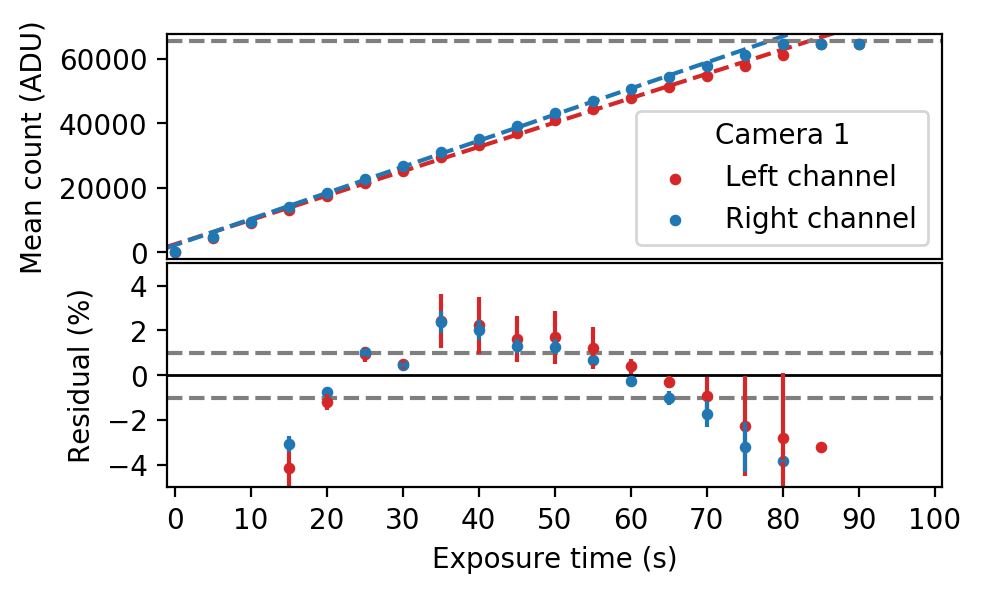
\includegraphics[width=\linewidth]{images/detectors/lin_1.png}
        \end{minipage}
        \begin{minipage}[t]{0.47\textwidth}\vspace{10pt}
            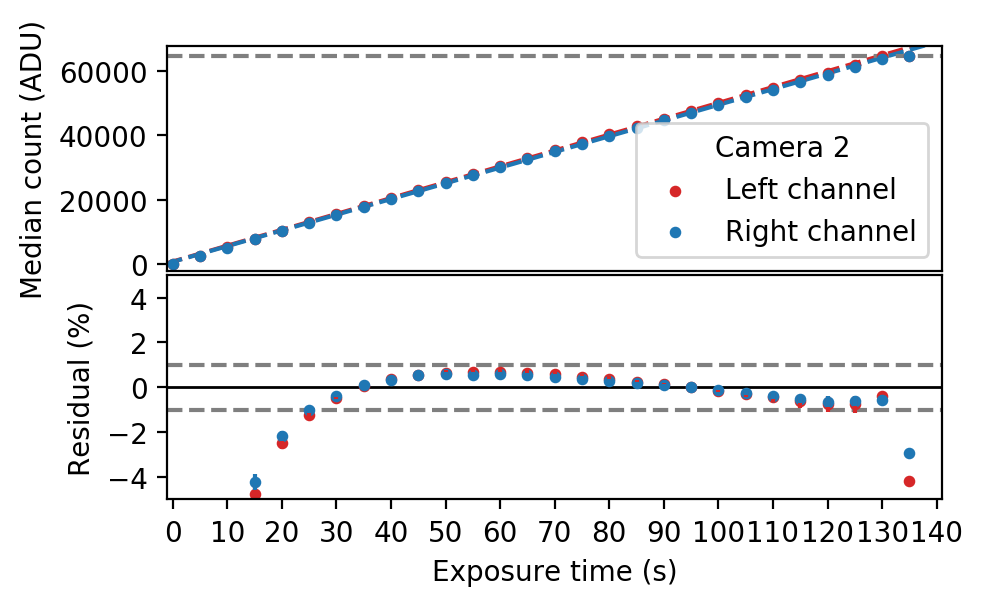
\includegraphics[width=\linewidth]{images/detectors/lin_2.png}
        \end{minipage}

        \begin{minipage}[t]{0.47\textwidth}\vspace{10pt}
            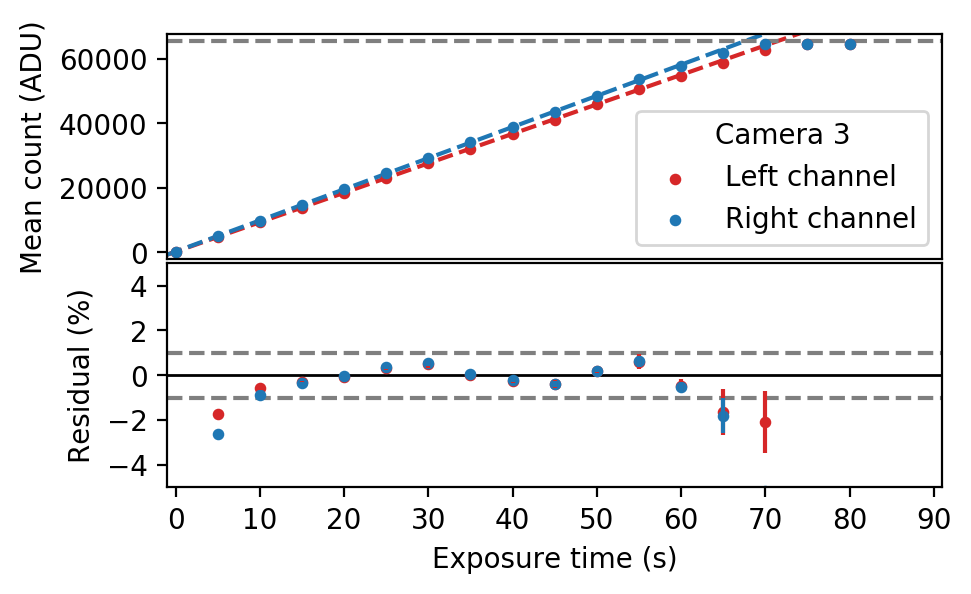
\includegraphics[width=\linewidth]{images/detectors/lin_3.png}
        \end{minipage}
        \begin{minipage}[t]{0.47\textwidth}\vspace{10pt}
            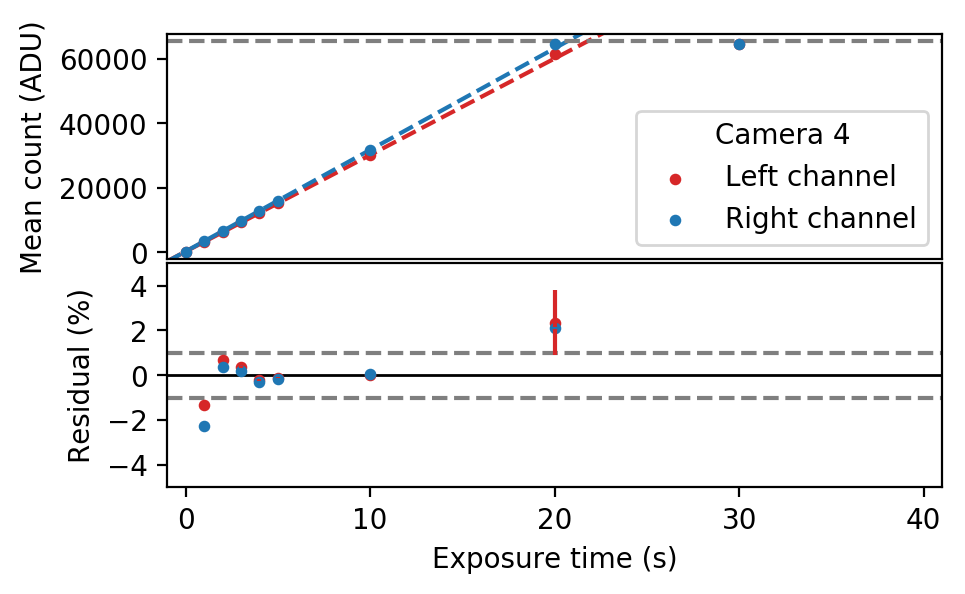
\includegraphics[width=\linewidth]{images/detectors/lin_4.png}
        \end{minipage}

        \begin{minipage}[t]{0.47\textwidth}\vspace{10pt}
            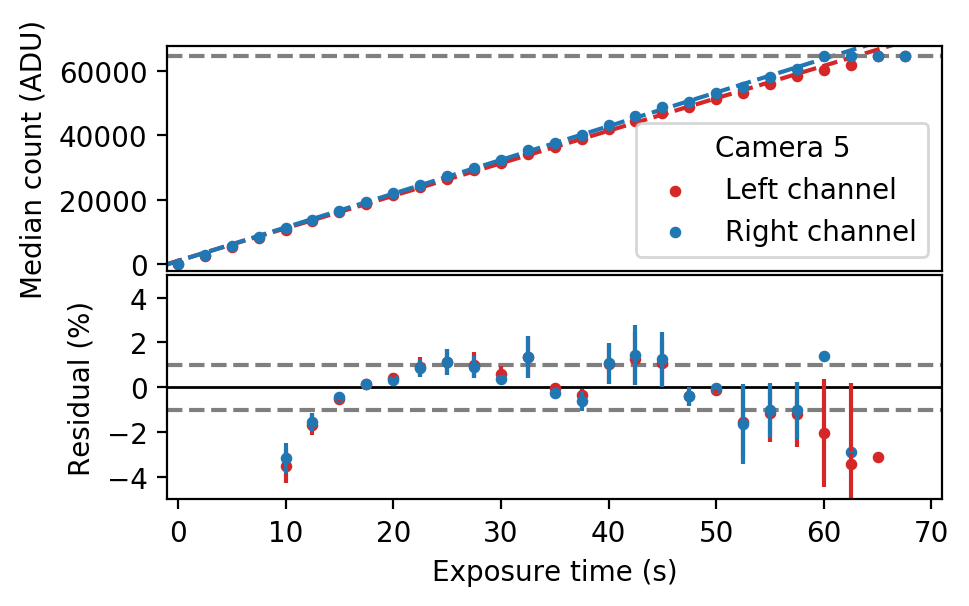
\includegraphics[width=\linewidth]{images/detectors/lin_5.png}
        \end{minipage}
        \begin{minipage}[t]{0.47\textwidth}\vspace{10pt}
            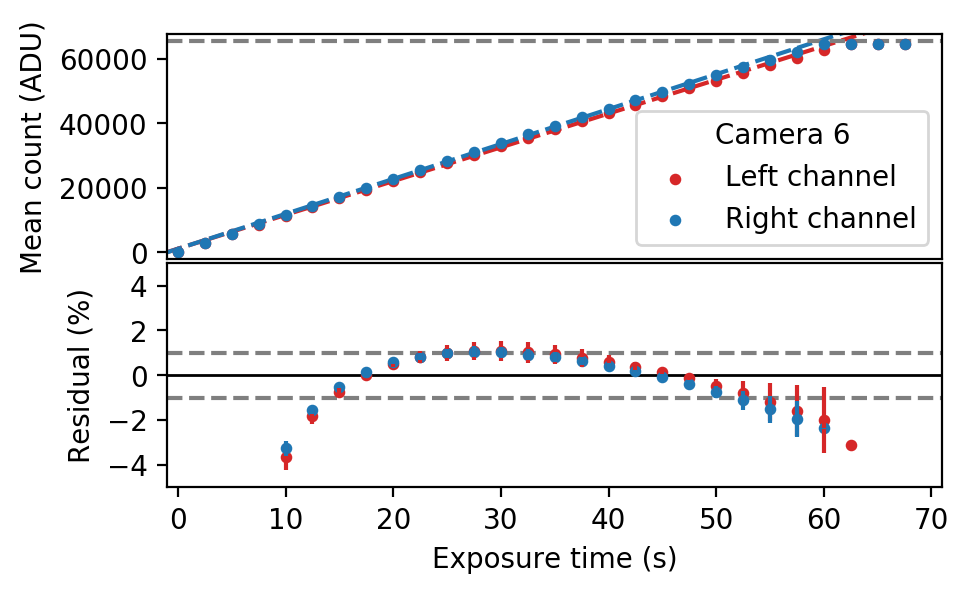
\includegraphics[width=\linewidth]{images/detectors/lin_6.png}
        \end{minipage}

        \begin{minipage}[t]{0.47\textwidth}\vspace{10pt}
            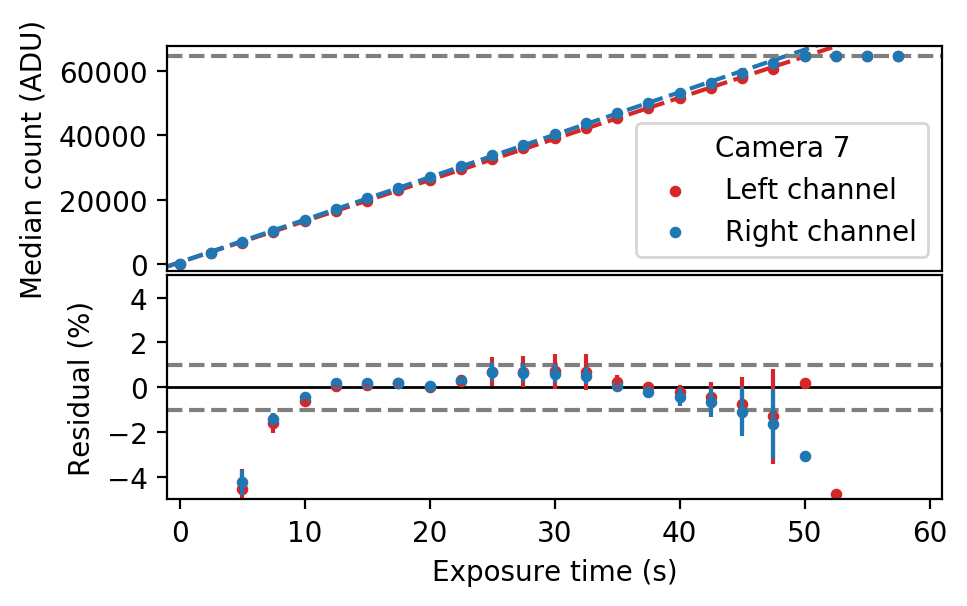
\includegraphics[width=\linewidth]{images/detectors/lin_7.png}
        \end{minipage}
        \begin{minipage}[t]{0.47\textwidth}\vspace{10pt}
            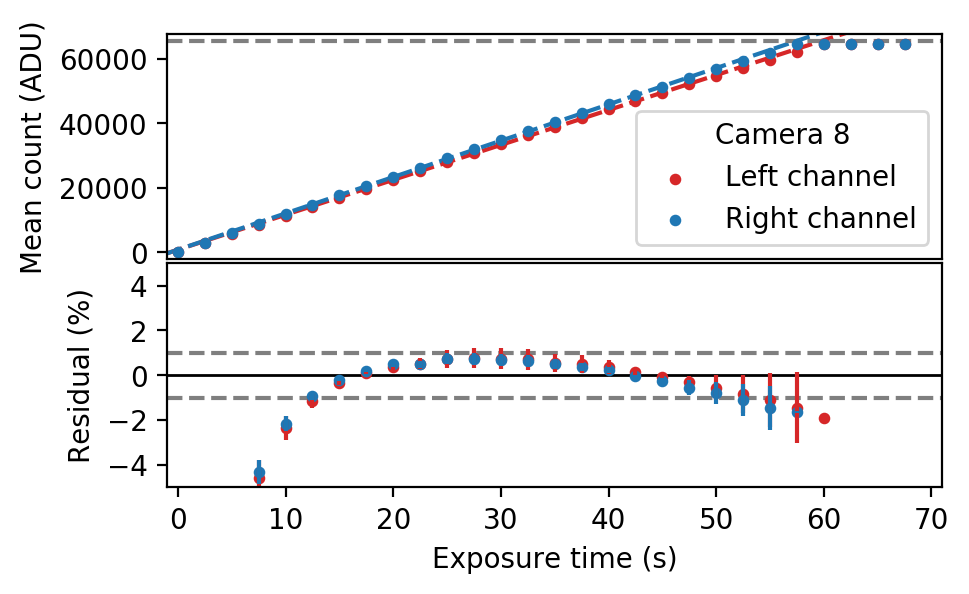
\includegraphics[width=\linewidth]{images/detectors/lin_8.png}
        \end{minipage}
    \end{center}
    \caption[Linearity plots]{
        Linearity plots for each camera. The horizontal dashed line in the top panel shows the saturation level from \aref{tab:ptc}, and the dashed lines in the lower panels show the target $\pm$1\% non-linearity range.
    }\label{fig:lin}
\end{figure}

\clearpage

\end{colsection}

% ~~~~~~~~~~~~~~~~~~~~
\newpage
\subsection{Defects}
\label{sec:defects}
\begin{colsection}

There are several possible defects in CCD sensors \citep{CCDs}: hot pixels, which have atypically high dark currents, dead pixels, which produce low or zero counts, and trap pixels, which ``trap'' electrons and prevent read out from it and any pixels above it in the column. It is important to identify any bad pixels so that the GOTOphoto pipeline (see \aref{sec:gotophoto}) can mask them when reducing the images from each camera.

Single hot or dead pixels can be removed to some extent by subtracting dark frames and flat fielding. Trap pixels are more of an issue, as they can take out up to the entire column. For each camera a defect mask was made by taking the ratio of two flat field images with different exposure times, making any bad columns easy to pick out by comparing to the surrounding pixels. An example of a bad column caused by a trap pixel is shown in \aref{fig:itsatrap}. The positions of bad columns for each camera are given in \aref{tab:traps}. The KAF-50100 chip specification gives an allowed limit of less than 20 column defects per device, which the GOTO cameras are well within.

\begin{table}[t]
    \begin{center}
        \begin{tabular}{c|ccc} %chktex 44
             & \multicolumn{2}{c}{Trap location} & Height \\
             & x & y & \% \\
            \midrule
            Camera 1 & 7751 & 4361 & 30 \\
            Camera 2 & 1658 & ~172 & 97 \\ %chktex 39
            Camera 3 & 1224 & 1844 & 70 \\
                     & 5058 & 5185 & 17 \\
            Camera 4 & 5406 & 2607 & 58 \\
            Camera 5 & 6293 & 1416 & 77 \\
            Camera 6 & 5455 & 5036 & 19 \\
        \end{tabular}
        \hspace{0.5cm}
        \begin{tabular}{c|ccc} %chktex 44
            & \multicolumn{2}{c}{Trap location} & Height \\
            & x & y & \% \\
            \midrule
            Camera 7 & 1344 & 3037 & 51 \\
                     & 2326 & 2495 & 60 \\
                     & 2610 & 5688 & ~9 \\ %chktex 39
                     & 7491 & 5120 & 18 \\
            Camera 8 & 1184 & 3043 & 51 \\
                     & 5659 & 2778 & 55 \\
            \multicolumn{4}{c}{} \\
        \end{tabular}
    \end{center}
    \caption[Locations of bad columns]{
        Locations and extent (as a percentage of the total column height) of bad columns for each camera.
    }\label{tab:traps}
\end{table}

\begin{figure}[p]
    \begin{center}
        \includegraphics[width=\textwidth]{images/detectors/defect_plot.pdf}
    \end{center}
    \caption[An example of a column defect]{
        A flat field for Camera 1 showing a bad column. The location of the trap pixel is magnified, showing that the pixels in the column above the trap have been prevented from being read out. The bad column is also also clearly visible in the plot below, which shows the average counts in each column.
    }\label{fig:itsatrap}
\end{figure}

\clearpage

\end{colsection}

% ~~~~~~~~~~~~~~~~~~~~

\end{colsection}

% ########################################

\newpage
\section{System throughput}
\label{sec:throughput}
\begin{colsection}

% ~~~~~~~~~~~~~~~~~~~~

\begin{colsection}

Unfortunately, not every photon emitted by a target object will be recorded by a telescope: photons will be lost due to absorption and scattering in the Earth's atmosphere, and within the telescope's optics and camera. Understanding each of these factors is required in order to produce a complete throughput model, which can then be compared to the real system (in \aref{sec:onsky_comparison}) to see if the hardware is performing as expected.

\end{colsection}

% ~~~~~~~~~~~~~~~~~~~~
\subsection{Optical elements}
\label{sec:optics}
\begin{colsection}

As described in \aref{sec:goto_design}, the GOTO unit telescopes are Wynne-Newtonian astrographs: fast (f/2.5) Newtonian telescopes with a \SI{40}{\centi\meter} primary mirror, a flat elliptical secondary (\SI{19}{\centi\metre} short axis) and a Wynne corrector between the secondary and the camera. A drawing of the \glsfirst{ota} is shown in \aref{fig:ota}, and the five elements the light must pass through (the three corrector lenses, the filter in the filter wheel and the window in front of the detector) are shown in \aref{fig:wynne}. In order to model the throughput each element needed to be considered in turn.

% ---------
\subsubsection{Mirrors}

The GOTO mirrors are were manufactured by Orion Optics\footnote{\url{https://www.orionoptics.co.uk/}}. Orion used their own ``HiLux'' high reflectivity aluminium coating, and while individual reflectance curves were not available for the GOTO mirrors at the time this work was carried out, Orion did provide a representative reflectance curve on their website (shown in \aref{fig:trans_ota}). As there are two mirrors this curve will be included twice in the final throughput model. The difference in the angle of incidence of light on the two mirrors is accounted for in the coating applied to each mirror, so the reflectivity curves of the two are assumed to be identical.

\newpage

\begin{figure}[p]
    \begin{center}
        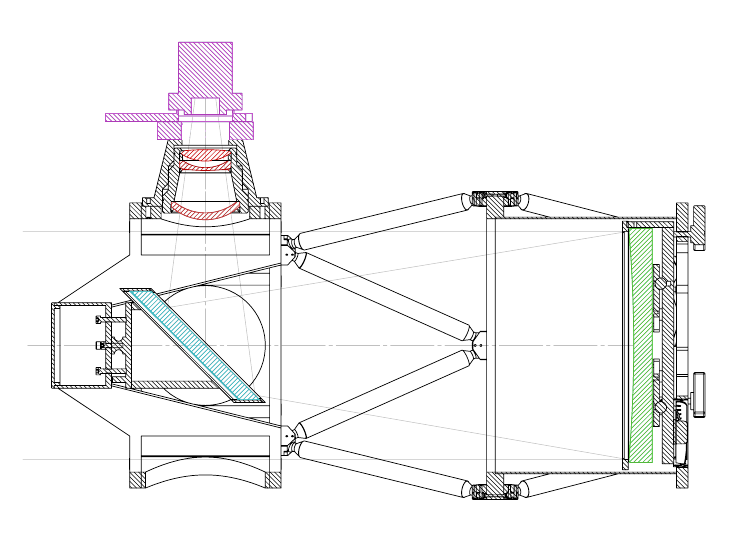
\includegraphics[width=0.7\textwidth]{images/throughput/OTA_optics.png}
    \end{center}
    \caption[GOTO optical telescope assembly]{
        The \glsfirst{ota} design for one of the GOTO unit telescopes. Light enters from the left, and relevant elements have been highlighted: the primary mirror in \textcolorbf{Green}{green}, the secondary mirror in \textcolorbf{BlueGreen}{blue}, the Wynne corrector in \textcolorbf{Red}{red} and the FLI camera hardware in \textcolorbf{Purple}{purple}.
    }\label{fig:ota}
\end{figure}

\begin{figure}[p]
    \begin{center}
        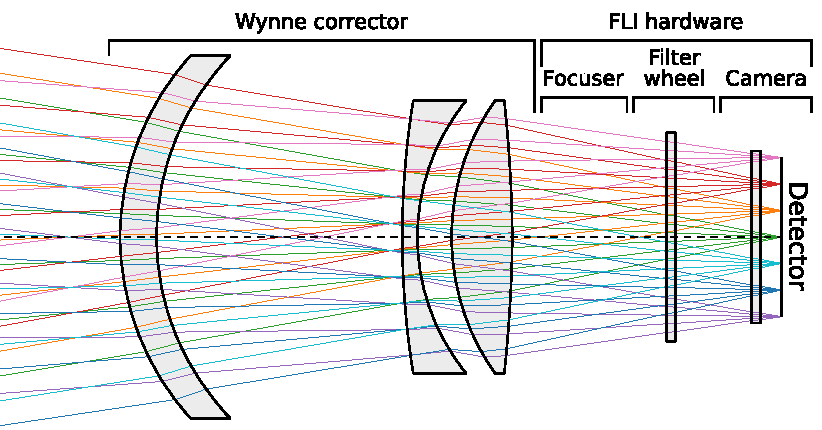
\includegraphics[width=0.7\textwidth]{images/throughput/wynne.pdf}
    \end{center}
    \caption[Ray tracing the corrector elements]{
        A ray trace through the optical elements after the primary and secondary mirrors. From left-to-right light passes through the three Wynne corrector lenses, the filter, and the camera window before reaching the detector located in the focal plane.
    }\label{fig:wynne}
\end{figure}

\clearpage

% ---------
\subsubsection{Lenses}

\begin{table}[t]
    \begin{center}
        \begin{tabular}{c|ccccc|c} %chktex 44
                 &       &                        & \multicolumn{2}{c}{Radius of curvature}         & On-axis               & Glass \\
            Lens & Shape & Diameter               & Exterior               & Interior               & thickness             & type \\
            \midrule
            1 & Meniscus & \SI{120}{\milli\metre} &  \SI{89}{\milli\metre} &  \SI{86}{\milli\metre} & \SI{12}{\milli\metre} & H-K9L   \\
            2 & Meniscus &  \SI{90}{\milli\metre} & \SI{278}{\milli\metre} &  \SI{71}{\milli\metre} &  \SI{5}{\milli\metre} & H-K9L   \\
            3 & Biconvex &  \SI{90}{\milli\metre} &  \SI{77}{\milli\metre} & \SI{378}{\milli\metre} & \SI{20}{\milli\metre} & S-FPL53 \\
        \end{tabular}
    \end{center}
    \caption[Wynne corrector lens properties]{
        Properties of the three Wynne corrector lenses.
    }\label{tab:lenses}
\end{table}

Each Wynne corrector contains three lenses, as shown in \aref{fig:wynne} --- the details of each lens are given in \aref{tab:lenses}. No complete transmission data was available, so a model throughput curve had to be created.

For each lens the reflectivity of the front and rear surfaces and the internal transmittance of the glass needs to be considered. Each surface is coated with an anti-reflection coating, the profile of which was included in the GOTO optical report. Transmittance curves for each lens were not available, but the glass types were included in the report and are given in \aref{tab:lenses}. Transmittance data provided by the glass manufacturers were retrieved from the online Refractive Index Database\footnote{\url{https://refractiveindex.info/}}. For simplicity, each lens was modelled as having a constant thickness, using their on-axis thickness. As shown in \aref{fig:wynne}, this is a good approximation for lens 1 but will underestimate the absorption within lens 2 and overestimate the absorption within lens 3.

Throughput curves for the anti-reflection coatings and the glass for the three lenses are shown in \aref{fig:trans_lenses} along with the total throughput of the corrector, found by multiplying the contributions from the glass transmission and the coating on both surfaces of each lens:
%
\begin{equation}
    T_\text{corrector} = T_\text{Lens1} \times
                         T_\text{Lens2} \times
                         T_\text{Lens3} \times
                         {(T_\text{coating})}^6.
    \label{eq:corrector}
\end{equation}

\newpage

\begin{figure}[t]
    \begin{center}
        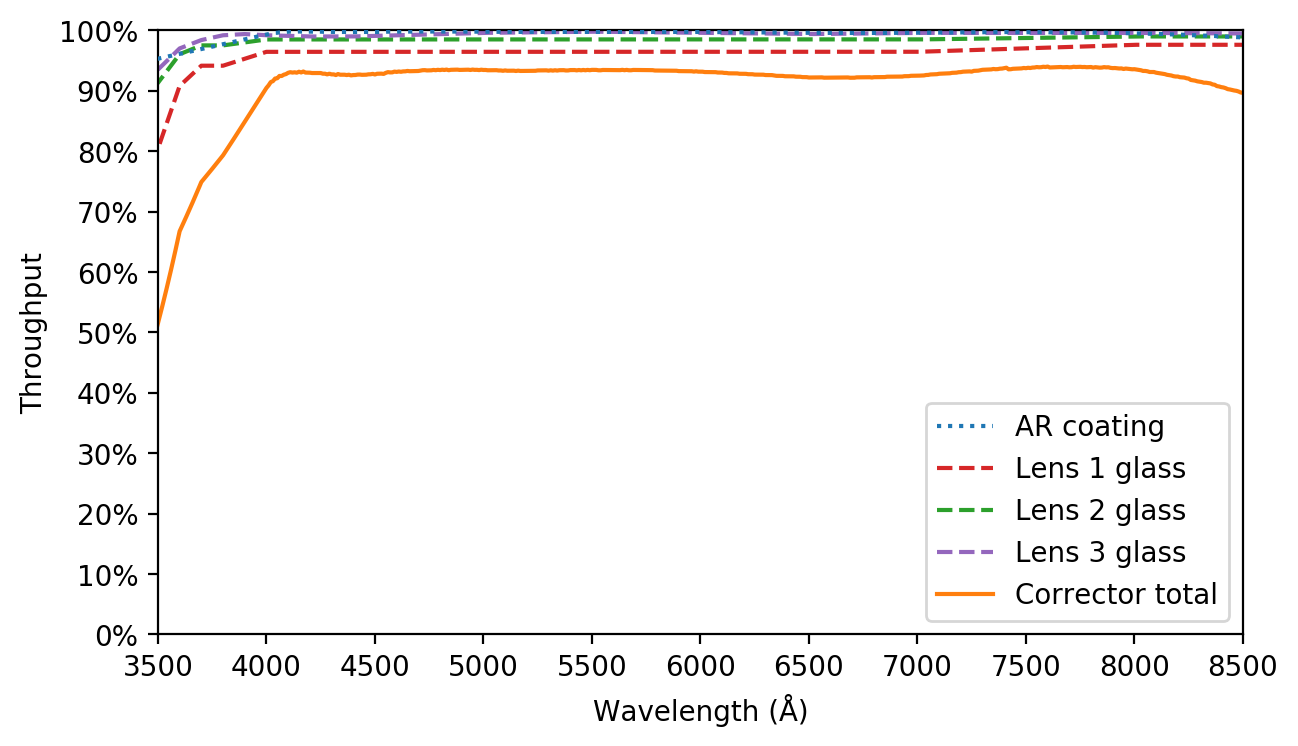
\includegraphics[width=\textwidth]{images/throughput/trans_lenses.png}
    \end{center}
    \caption[Wynne corrector transmission curve]{
        Transmission curve for the Wynne corrector (the \textcolorbf{Orange}{orange} solid line), comprised of the glass throughput of each lens (\textcolorbf{Red}{red}, \textcolorbf{Green}{green} and \textcolorbf{Purple}{purple} dashed lines) and an anti-reflection (AR) coating on all six surfaces (\textcolorbf{NavyBlue}{blue} dotted line).
    }\label{fig:trans_lenses}
\end{figure}

% ---------
\subsubsection{Filters}

The filter transmittance is included in their bandpass profiles, described below in \aref{sec:filters}. At this stage we will consider the OTA with no filter, so as to produce an unfiltered OTA transmission curve which can then by multiplied by the chosen filter bandpass.

% ---------
\subsubsection{Camera window}

Finally, before reaching the detector, light must pass through a glass window in the camera which protects the CCD sensor. The window is made of F116 glass, and a transmission profile was provided by FLI.\@ This is shown in \aref{fig:trans_ota}.

\newpage

% ---------
\subsubsection{Combined OTA throughput}

The combined throughput for the whole unfiltered OTA is shown in \aref{fig:trans_ota}. This was constructed by multiplying through the transmission curves for the two mirrors, the corrector (from \aref{eq:corrector}) and the camera window:
%
\begin{equation}
    T_\text{OTA} = {(T_\text{mirror})}^2 \times T_\text{corrector} \times T_\text{window}.
    \label{eq:ota}
\end{equation}
%
In the 4000--\SI{7000}{\angstrom} visible region used by GOTO the throughput is typically 60\% or above, although all the elements have a sharp cut-off towards the blue.

\begin{figure}[t]
    \begin{center}
        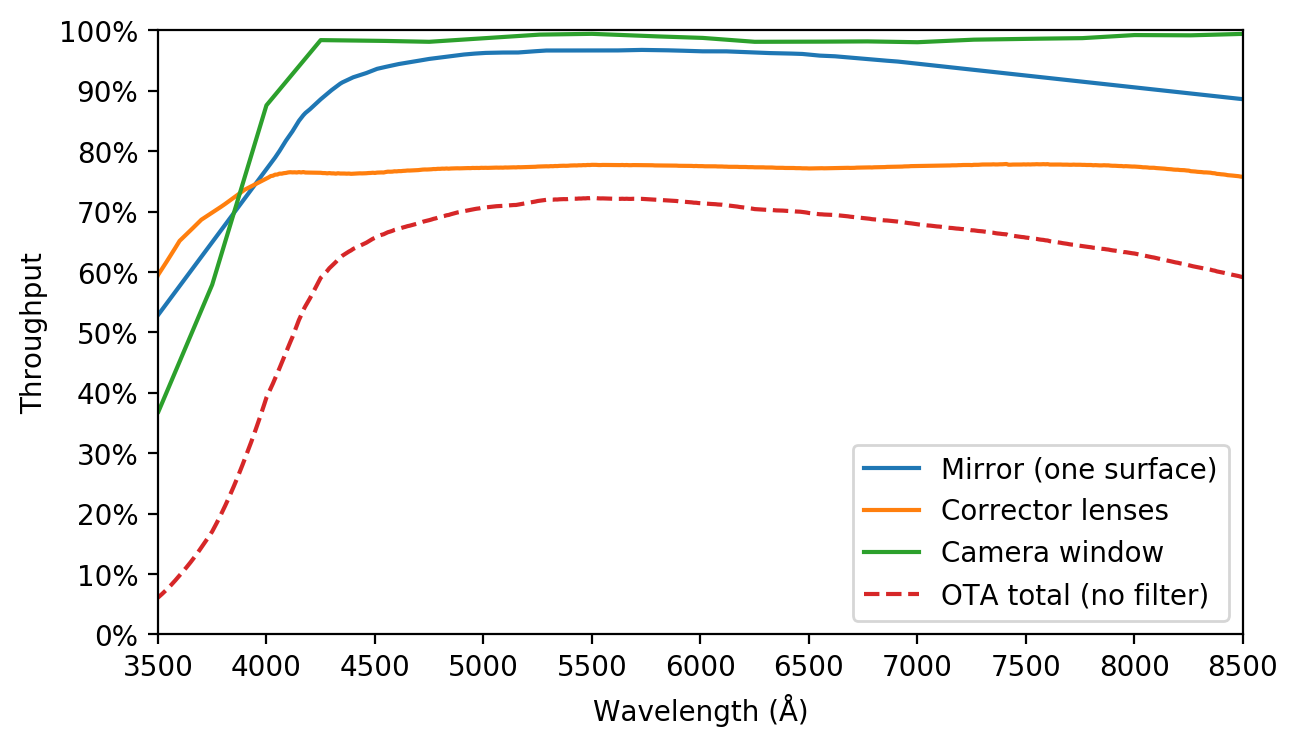
\includegraphics[width=\textwidth]{images/throughput/trans_ota.png}
    \end{center}
    \caption[Combined OTA transmission curve]{
        Transmission curve for the unfiltered OTA (the \textcolorbf{Red}{red} solid line), which includes the two mirrors (\textcolorbf{NavyBlue}{blue} dashed line), the combination of all three corrector lenses (\textcolorbf{Orange}{orange} dashed line, from \aref{fig:trans_lenses}) and the camera window (\textcolorbf{Green}{green} dashed line).
    }\label{fig:trans_ota}
\end{figure}

\end{colsection}

% ~~~~~~~~~~~~~~~~~~~~
\newpage
\subsection{Filters}
\label{sec:filters}
\begin{colsection}

\begin{figure}[t]
    \begin{center}
        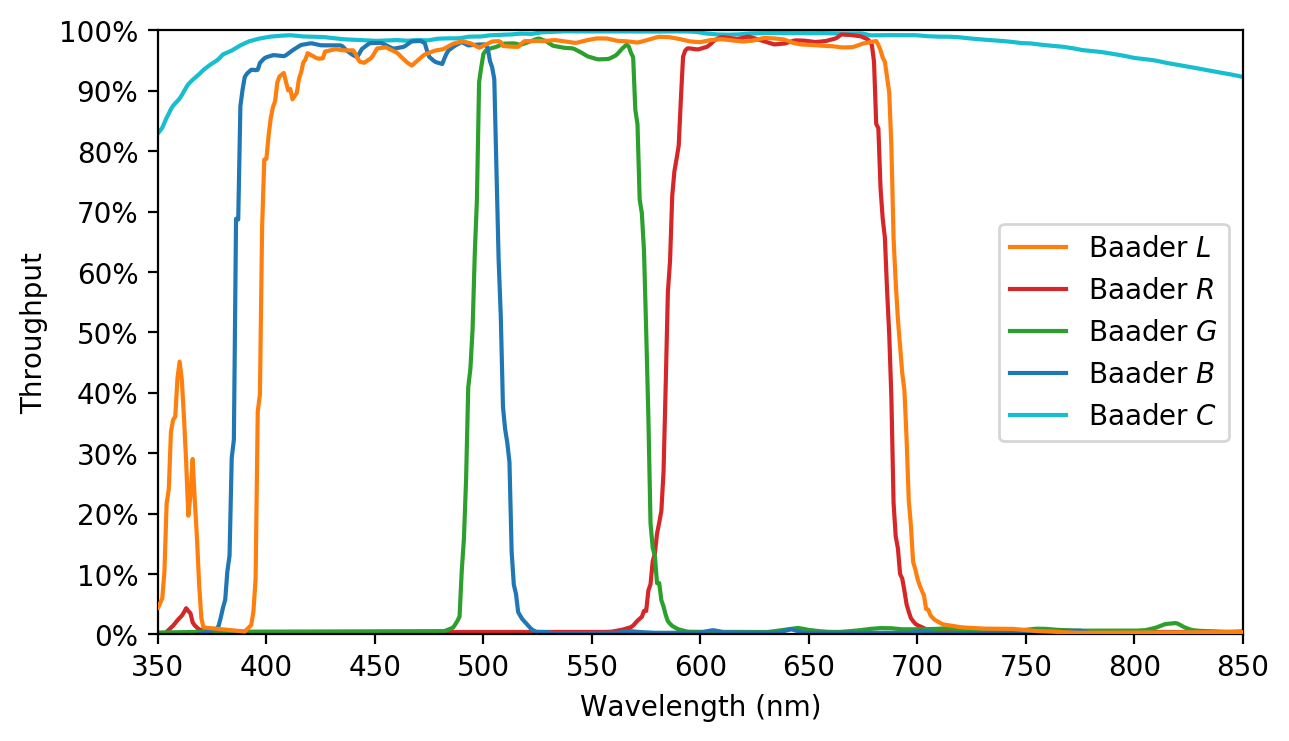
\includegraphics[width=\textwidth]{images/throughput/trans_filters.png}
    \end{center}
    \caption[Baader filter transmission curves]{
        Transmission curves for the Baader \textit{LRGBC} filter set used by GOTO.\
    }\label{fig:filters}
\end{figure}

Each GOTO unit telescope has a five-slot filter wheel containing a set of \SI{65}{\milli\metre} square filters from Baader Planetarium\footnote{\url{https://www.baader-planetarium.com}}: three coloured filters (\textit{R}, \textit{G}, \textit{B}), one wide ``luminance'' filter (\textit{L}) covering the whole visible range, and a clear glass filter ({\textit{C}}). Transmission curves for each filter are shown in \aref{fig:filters}. Each filter has a high throughput and steep cut-offs outside of the desired bandpasses. For the coloured filters the cut-offs were chosen so the [O\textsc{iii}] $\lambda 5007$ emission line falls within the overlap of the \textit{B} and \textit{G} filters and the region around \SI{5800}{\angstrom}, which contains emission lines from Mercury and Sodium vapour lamps, is excluded by the gap between the \textit{G} and \textit{R} filters.

Most GOTO observations are taken using the \textit{L} filter, however the \textit{RGB} filters have been used for manual follow-up observations. The clear filter is never used for scientific observations, so it is not considered as part of the throughput model going forward.

\begin{table}[t]
    \begin{center}
        \begin{tabular}{c|cccc} %chktex 44
             & Effective wavelength & Effective bandwidth\\
            Filter & ($\lambda_\text{eff}$, \SI{}{\angstrom}) & ($\Delta\lambda$, \SI{}{\angstrom}) \\
            \midrule
            Baader \textit{L} & 5355 & 2942 \\
            Baader \textit{R} & 6573 &  979 \\
            Baader \textit{G} & 5373 &  813 \\
            Baader \textit{B} & 4509 & 1188 \\
        \end{tabular}
    \end{center}
    \caption[Baader filter properties]{
        Properties of the Baader \textit{LRGB} filters.
    }\label{tab:filters}
\end{table}

Properties of the \textit{LRGB} filters are given in \aref{tab:filters}. The effective wavelength ($\lambda_\text{eff}$) is the pivot wavelength as defined in \citet{HST_calibration} for HST filters:
%
\begin{equation}
    \lambda_\text{eff}^2 = \frac{\int T\lambda~d\lambda}{\int T/\lambda~d\lambda},
    \label{eq:pivot_wavelength}
\end{equation}
%
where $T$ is the transmission integrated over all wavelengths $\lambda$. The effective bandwidth ($\Delta\lambda$) is found by calculating the equivalent width, the width of a rectangle that has a height equal to the maximum transmission (unity) and the same area as the area under the filter transmission curve, i.e. \todo{Ask Vik}
%
\begin{equation}
    \Delta\lambda = \int T~d\lambda.
    \label{eq:bandwidth}
\end{equation}

The Baader filters were designed for amateur astronomers and astro-photographers and are less commonly used by professional instruments than other sets, such as the \textit{u'g'r'i'z'} set used by the Sloan Digital Sky Survey \glsadd{sdss} \citep{Sloan_filters} or the traditional Johnson-Cousins \textit{UBVRI} set redefined by \citet{Bessell_filters}. GOTO primarily uses Baader filters to reduce costs, as each unit telescope requires a full set. A comparison of the Baader \textit{LRGB} transmission curves with Sloan are shown in \aref{fig:filter_comparison1} and with Bessell \aref{fig:filter_comparison2}. The Baader \textit{L} filter approximately covers the Sloan \textit{g'} and \textit{r'} filters, the \textit{B} and \textit{G} filters cover \textit{g'} and \textit{R} roughly matches \textit{r'}. Colour terms to compare GOTO \textit{RGB} observations with Sloan \textit{g'} and \textit{r'} observations were calculated by \citet{Phaethon}.

\newpage

\begin{figure}[t]
    \begin{center}
        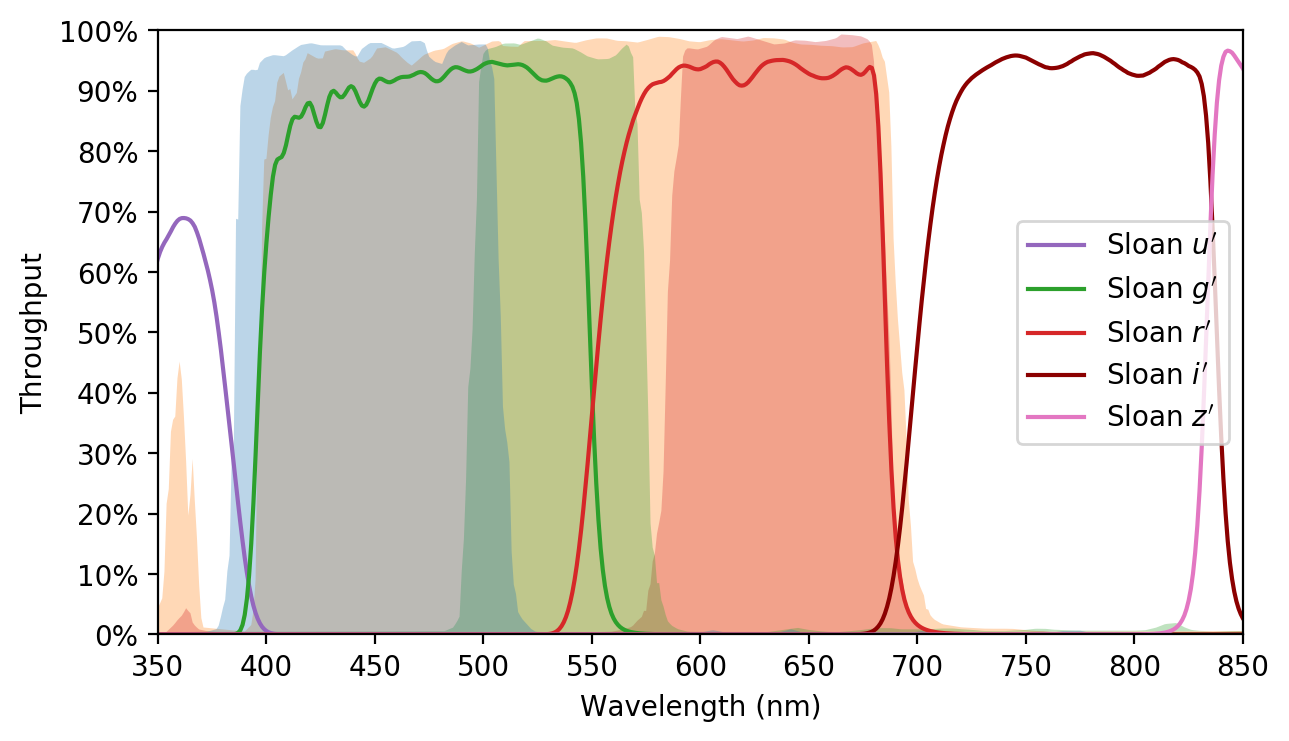
\includegraphics[width=\textwidth]{images/throughput/filt_comp1.png}
    \end{center}
    \caption[Comparison of Baader and Sloan filters]{
        A comparison of the Baader \textit{LRGB} filters to the Sloan \textit{u'g'r'i'z'} set.
    }\label{fig:filter_comparison1}
\end{figure}

\begin{figure}[t]
    \begin{center}
        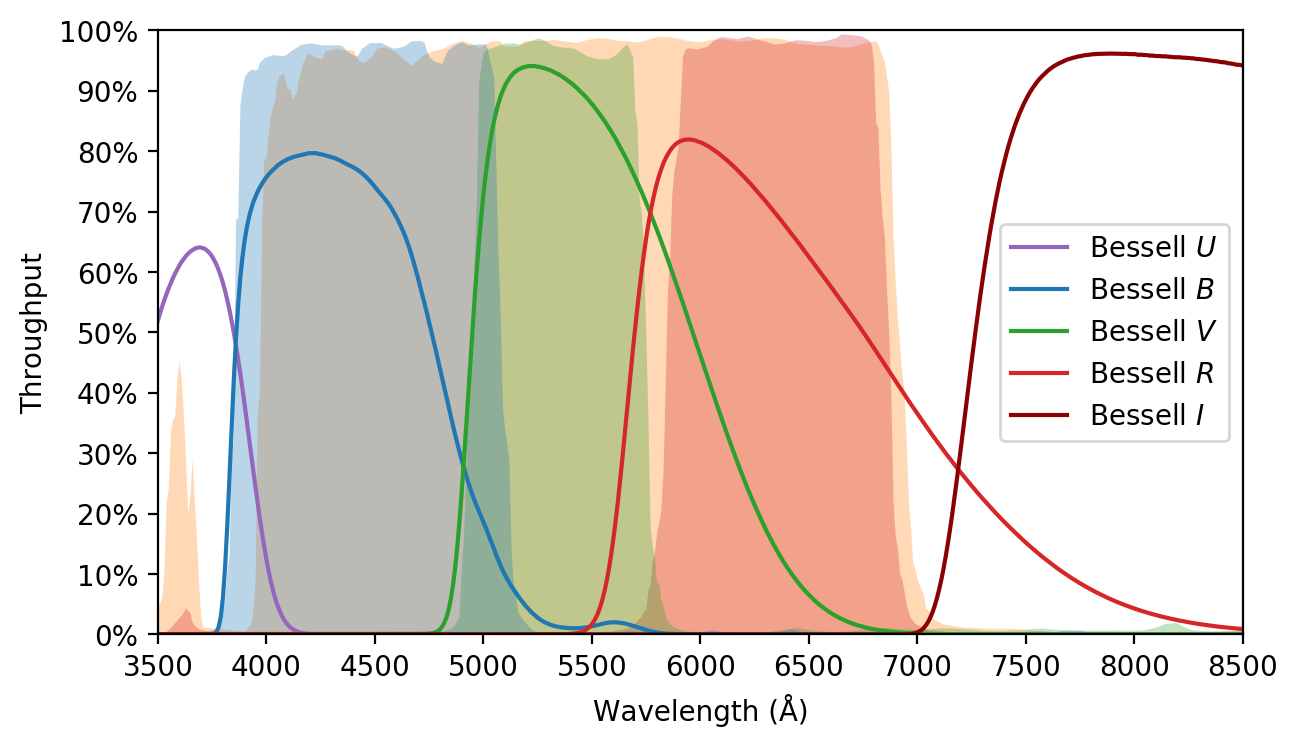
\includegraphics[width=\textwidth]{images/throughput/filt_comp2.png}
    \end{center}
    \caption[Comparison of Baader and Bessell filters]{
        A comparison of the Baader \textit{LRGB} filters to the Bessell \textit{UBVRI} set.
    }\label{fig:filter_comparison2}
\end{figure}

\clearpage

\end{colsection}

% ~~~~~~~~~~~~~~~~~~~~
\newpage
\subsection{Quantum efficiency}
\label{sec:qe}
\begin{colsection}

\begin{figure}[t]
    \begin{center}
        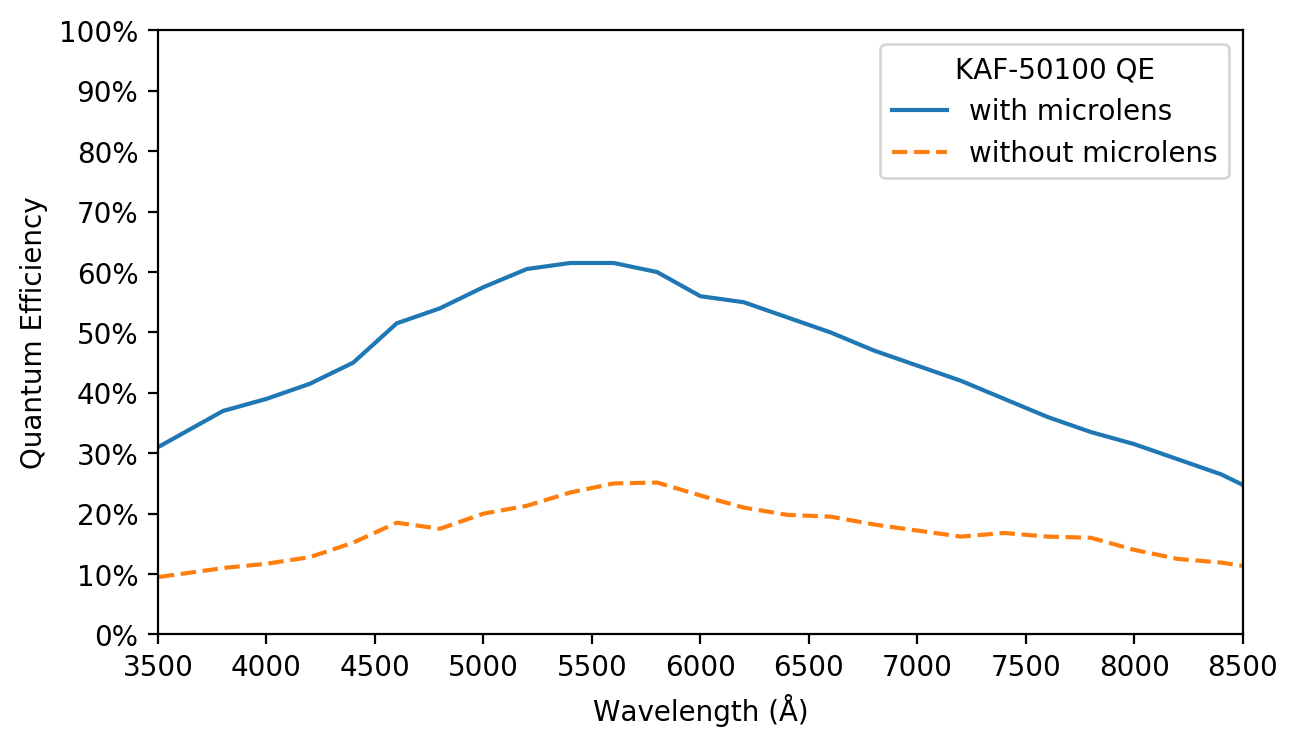
\includegraphics[width=\textwidth]{images/throughput/qe.png}
    \end{center}
    \caption[CCD quantum efficiency curve]{
        Quantum efficiency curve for the KAF-50100 CCDs.
    }\label{fig:qe}
\end{figure}

Once photons pass through the telescope optics they are focused onto the CCD, where they interact with the photosensitive layer and produce electric charge carriers which are recorded by the detector \citep{CCDs}. The conversion from photons to electrons is measured by the \glsfirst{qe} of the CCD and is dependent on wavelength: short-wavelength photons will be absorbed before reaching the photosensitive layer, while long wavelength photons will not have enough energy to create free electrons in the silicon. CCDs that are back-side illuminated have improved blue QE due to each photon not having to pass through the electrode layer and therefore having less chance of being absorbed, however these are more complicated and expensive to build. The QE of a CCD can also change as a function of temperature, but this is negligible in the visible portion of the spectrum. The QE curve for the (front-illuminated) KAF-50100 CCDs within the cameras used by GOTO is shown in \aref{fig:qe}.

\end{colsection}

% ~~~~~~~~~~~~~~~~~~~~
\newpage
\subsection{Total throughput}
\label{sec:total_throughput}
\begin{colsection}

\begin{figure}[t]
    \begin{center}
        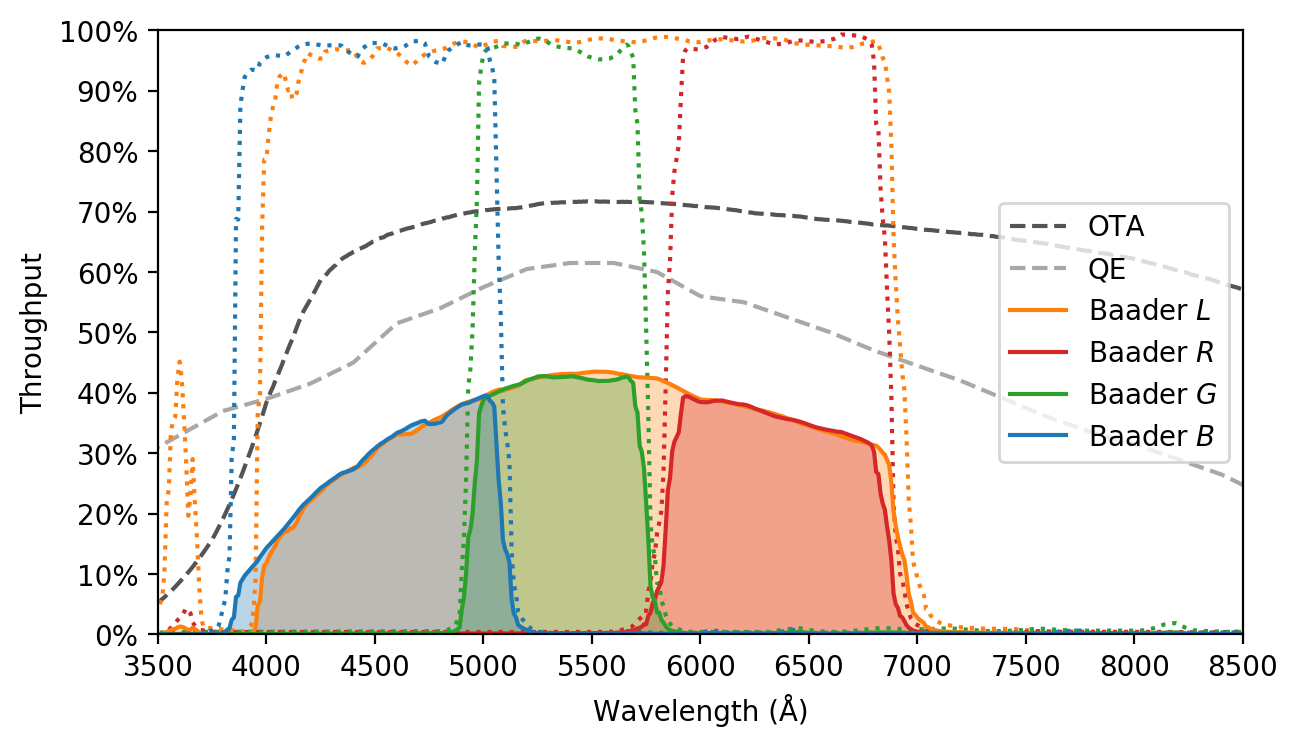
\includegraphics[width=\textwidth]{images/throughput/throughput.png}
    \end{center}
    \caption[Complete throughput model for the GOTO filters]{
        The complete GOTO throughput model. The model elements (dashed lines) are the throughput of the OTA elements (from \aref{fig:trans_ota}) and the quantum efficiency of the CCD (from \aref{fig:qe}); and the Baader \textit{LRGB} filter bandpasses (from \aref{fig:filters}) are shown by the coloured dotted lines. The filled lines shown the total throughput in each filter when the model is applied.
    }\label{fig:throughput}
\end{figure}

The complete GOTO throughput is a combination of all of the elements discussed in the previous sections. Each source profile was linearly interpolated to the same wavelength range (3500--\SI{8500}{\angstrom}) and multiplied together to produce the total GOTO throughput model, shown in \aref{fig:throughput}. Since the quantum efficiency has been included, the total throughput describes the conversion between photons above the atmosphere to electrons detected in the CCD, and using the gain values given in \aref{tab:ptc} the full conversion between photons and output counts can be made. The mean throughput in each filter can be found by dividing the filled areas in \aref{fig:throughput} by the area of the filter bandpass, and are given in electrons per photon in \aref{tab:throughput_extinction}.

\end{colsection}

% ~~~~~~~~~~~~~~~~~~~~
\newpage
\subsection{Atmospheric extinction}
\label{sec:atmosphere}
\begin{colsection}

\begin{figure}[t]
    \begin{center}
        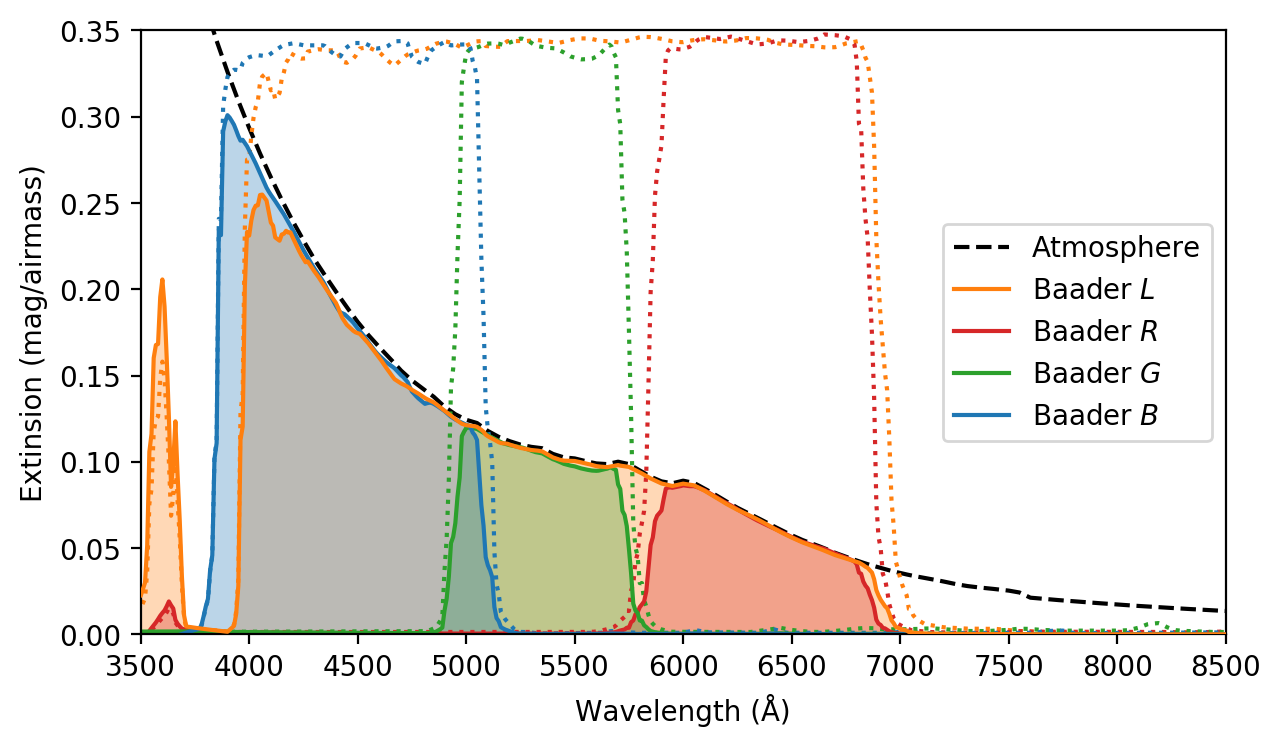
\includegraphics[width=\textwidth]{images/throughput/ext.png}
    \end{center}
    \caption[Atmospheric extinction in the GOTO filters]{
        Atmospheric extinction in the GOTO filters, in magnitude per airmass. The measured extinction curve from \citet{tn31} is shown by the black dashed line, and the filled lines show the extinction curve multiplied by the filter bandpasses from \aref{fig:filters} (shown by the coloured dotted lines).
    }\label{fig:extinction}
\end{figure}

In order to model the entire light path from an astronomical source through to the CCD detector the absorption of light by the Earth's atmosphere must also be considered. The atmosphere is close to transparent over most of the visible region, however losses due to Rayleigh scattering begin to dominate closer to the UV \citep{atmosphere}.

The amount of light lost due to absorption and scattering in the atmosphere will depend on the altitude of the source, as light from sources closer to the horizon will pass a denser airmass. The extinction of the atmosphere above La Palma has been measured in terms of magnitude per source airmass by \citet{tn31}, and is shown in \aref{fig:extinction}.

\newpage

Atmospheric extinction can be treated like the throughput elements considered in \aref{sec:total_throughput}, except it is not included in the throughput model as it is not a function of the GOTO hardware. For the \textit{LRGB} filters the mean extinction can be found by multiplying the extinction curve by the filter bandpasses, as shown in \aref{fig:extinction}, and then dividing the filled areas under each curve by the area of the unmodified filter bandpass. These extinction values are given in magnitudes per airmass in \aref{tab:throughput_extinction}.

Another atmospheric factor unique to observing from La Palma is the \textit{calima}, large quantities of sand and dust from the Sahara Desert which can be carried over the site by westerly winds. The calima occurs most often in the summer, and analysis of dust-affected images has shown that the additional extinction is not wavelength dependent \citep{ORM_dust}. The extinction curve measured by \citep{tn31} was based on observations taken on dust-free nights, and the values in \aref{tab:throughput_extinction} do not include any additional extinction to model the effects of the calima. Based on analysing archival images over 20 years, \citet{ORM_dust} suggests the calima can increase the extinction by approximately 0.04 mag/airmass.

\begin{table}[t]
    \begin{center}
        \begin{tabular}{c|cc} %chktex 44
                   & Throughput     & Extinction \\
            Filter & (\elec/photon) & (mag/airmass) \\
            \midrule
            Baader \textit{L} & 0.35 & 0.13 \\
            Baader \textit{R} & 0.38 & 0.07 \\
            Baader \textit{G} & 0.42 & 0.11 \\
            Baader \textit{B} & 0.25 & 0.20 \\
        \end{tabular}
    \end{center}
    \caption[Theoretical throughput and atmospheric extinction for the GOTO filters]{
        Theoretical throughputs and atmospheric extinction for the GOTO filters.
    }\label{tab:throughput_extinction}
\end{table}

\end{colsection}

% ~~~~~~~~~~~~~~~~~~~~

\end{colsection}

% ########################################

\newpage
\section{Photometric modelling}
\label{sec:photometry}
\begin{colsection}

% ~~~~~~~~~~~~~~~~~~~~

\begin{colsection}

Using the throughput model created in \aref{sec:throughput} it was possible to simulate photometric observations with GOTO before the telescope was commissioned. This section applies the theoretical throughput model to two important photometric properties: the magnitude zeropoint (the correction required to convert between instrumental and calibrated magnitude values) and the limiting magnitude (the faintest magnitude a source can be to still produce a detectable signal above a given noise threshold). These theoretical values are then compared to values calculated from real GOTO observations, in order to check that the hardware is performing to specification.

\end{colsection}

% ~~~~~~~~~~~~~~~~~~~~
\subsection{Magnitude zeropoints}
\label{sec:zeropoints}
\begin{colsection}

The output flux of a source, $F$, is related to its magnitude, $m$, by
%
\begin{equation}
    m = -2.5 \log_{10}(F).
    \label{eq:apparent_magnitude}
\end{equation}
%
In practice magnitudes, are usually measured relative to a reference star using
%
\begin{equation}
    m - m_\text{ref} = -2.5 \log_{10}\left(\frac{F}{F_\text{ref}}\right),
    \label{eq:magnitude_ref}
\end{equation}
%
which requires a reference star of known magnitude $m_\text{ref}$ and flux $F_\text{ref}$. Traditionally Vega is used as a reference star as it has a magnitude of very close to 0.

The instrumental magnitude measured from an image is related to the number of photo-electrons recorded, $N$, using the same magnitude definition
%
\begin{equation}
    \begin{split}
        m_\text{ins} & = -2.5 \log_{10}(N/t),
    \end{split}
    \label{eq:ins_mag}
\end{equation}
%
where $t$ is the exposure time. The number of photo-electrons recorded per second $N/t$ from a given source should be proportional to the source flux $F$ (assuming the camera has a low non-linearity, see \aref{sec:lin}). Relating the two through a constant $\kappa$ \aref{eq:ins_mag} becomes
%
\begin{equation}
    \begin{split}
        m_\text{ins} & = -2.5 \log_{10}\left(\kappa F\right) \\
                     & = -2.5 \log_{10}\left(F\right) - m_\text{ZP}    \\
                     & = m - m_\text{ZP},
    \end{split}
    \label{eq:ins_mag2}
\end{equation}
%
where constant $m_\text{ZP}$ is defined as the instrumental \emph{zeropoint}.

The zeropoint is so called because observing an object with a true magnitude equal to the zeropoint ($m = m_\text{ZP}$) will produce an instrumental magnitude of 0, which corresponds to one electron per second on the detector. The zeropoint is usually defined based on the electron rate that would be measured above the atmosphere, which allows zeropoints to be compared between telescopes. Each telescope and filter combination will have a unique zeropoint, and once determined it can be used to convert instrumental magnitudes measured using that telescope to the source magnitude using
%
\begin{equation}
    m = m_\text{ins} + m_\text{ZP}.
    \label{eq:zp}
\end{equation}
%
Therefore, were it possible to observe a star with $m=0$ (without saturating the detector) the zeropoint can be calculated as
%
\begin{equation}
    \begin{split}
        m_\text{ZP} & = 0 - m_\text{ins} \\
                    & = 2.5 \log_{10}(N/t).
    \end{split}
    \label{eq:zp2}
\end{equation}

\end{colsection}

% ~~~~~~~~~~~~~~~~~~~~
\newpage
\subsection{Calculating theoretical zeropoints}
\label{sec:model_zeropoints}
\begin{colsection}

Consider taking an observation of a zero magnitude star, such as Vega. From \aref{eq:zp}, the instrumental magnitude will be equal to the negative zeropoint. In the AB magnitude system a zero magnitude star has a fixed flux density $F_\nu = $ \SI{3631}{\jansky} \citep{Sloan_filters}. Therefore passing this flux through the throughput model for each filter created in \aref{sec:throughput} will produce a predicted signal in photo-electrons which can be used to calculate a theoretical zeropoint.

% ---------
\subsubsection{Estimating predicted counts from a 0 mag star}

First, the zero-magnitude flux density needs to be converted into a flux in photons. \SI{3631}{\jansky} is equal to \SI{3.631e-20}{\erg\per\second\per\centi\metre\squared\per\hertz}. To convert from $F_\nu$ to $F_\lambda$ this needs to be multiplied by a factor of $c/\lambda_\text{eff}^2$, where $c$ is the speed of light and $\lambda_\text{eff}$ is the effective wavelength of the photon, in this case the effective wavelength of the filter in question\footnote{The $c/\lambda_\text{eff}^2$ conversion factor comes from differentiating the relationship $\nu = c/\lambda$}. This will then give a flux in \si{\erg\per\second\per\centi\metre\squared\per\angstrom}, but to convert to a photon count it needs to be divided by the energy of each photon $E_\lambda$ given by
%
\begin{equation}
    \begin{split}
        E_\lambda = \frac{hc}{\lambda_\text{eff}},
    \end{split}
    \label{eq:photon_energy}
\end{equation}
%
where $h$ is Planck's constant. Again at this stage it is assumed that all of the photons have the effective wavelength of the filter. Therefore the expected flux in photons is given by
%
\begin{equation}
    \begin{split}
        F_\lambda = 1.51 \times 10^{26}/\lambda_\text{eff}~\si{\photon\per\second\per\centi\metre\squared\per\angstrom}
    \end{split}
    \label{eq:zero-mag_photons}
\end{equation}
%
where $\lambda_\text{eff}$ is given in Angstroms.

\newpage

\begin{table}[t]
    \begin{center}
        \begin{tabular}{c|cc|c} %chktex 44
                   & \multicolumn{2}{c|}{Zero-magnitude star} & \\
            Filter & flux       & predicted signal            & Zeropoint \\
                   & (photon/s) & (\elec/s)                   & (mag) \\
            \midrule
            Baader \textit{L} & \num{3.41e9} & \num{1.20e+09} & 22.70 \\
            Baader \textit{R} & \num{9.24e8} & \num{3.52e+08} & 21.37 \\
            Baader \textit{G} & \num{9.38e8} & \num{3.97e+08} & 21.50 \\
            Baader \textit{B} & \num{1.63e9} & \num{4.80e+08} & 21.70 \\
        \end{tabular}
    \end{center}
    \caption[Theoretical zeropoints for each of the GOTO filters]{
        The flux from a zero-magnitude star in each of the GOTO filters, along with the predicted signal and corresponding theoretical zeropoint found using the throughput model from \aref{sec:throughput}.
    }\label{tab:zeropoints}
\end{table}

Multiplying the value in \aref{eq:zero-mag_photons} by the effective filter bandwidth and the collecting area of the telescope will give the predicted photon flux in the detector. Each of GOTO's unit telescopes has a \SI{40}{\centi\metre} diameter primary mirror, however not all of this is available to collect photons due to the shadow cast by the secondary mirror. Assuming this blocks 10\% of the light gives an effective collecting area of \SI{1131}{\centi\metre\squared}. Using this and the filter properties given in \aref{tab:filters}, the theoretical flux in photons per second from a zero-magnitude star above the atmosphere can be calculated for each filter. These values are given in \aref{tab:zeropoints}.

Finally, multiplying the theoretical fluxes in \aref{tab:zeropoints} by the mean throughput values for each filter from \aref{tab:throughput_extinction} gives the predicted signal in detector in photo-electrons per second. Converting these signals into magnitudes using \aref{eq:ins_mag} gives the instrumental magnitude, and using \aref{eq:zp2} with $m=0$ gives the theoretical zeropoint. The predicted signals and zeropoints are also given in \aref{tab:zeropoints}.

\newpage

% ---------
\subsubsection{Modeling observations with pysynphot}

The above method is the typical way to calculate a theoretical zeropoint, but only approximates bandpasses of each filter by using the effective wavelength and bandwidth, and only considers the mean throughput instead of over the whole bandwidth. To account for the full bandpass a more robust model was created using the Python pysynphot module (Python Synthetic Photometry, \pkg{pysynphot})\footnote{\url{https://pysynphot.readthedocs.io/}}, which is based the IRAF \pkg{SYNPHOT} package. Each of the throughput elements described in \aref{sec:throughput} were imported to create throughput profiles for each filter, and observations were simulated of a flat spectrum of \SI{3631}{\jansky} (0 mag in the AB system) and the built-in Vega spectrum (0 mag in the Vega system) by multiplying the spectra with the bandpasses. The resulting spectra are shown in \aref{fig:pysynphot}; the area under each curve gives the predicted number of electrons produced by the zero-magnitude star in each system.

The predicted signals found using pysynphot, and the derived zeropoints, are given in \aref{tab:pysynphot_zeropoints}. The difference between the two photometric systems is visible, the AB spectrum gives more electrons in the red filter while the Vega spectrum is brighter in the blue (as shown in \aref{fig:pysynphot}).

\begin{table}[t]
    \begin{center}
        \begin{tabular}{c|cc|cc} %chktex 44
                   & \multicolumn{2}{c|}{AB system} & \multicolumn{2}{c}{Vega system}\\
            Filter & Signal    & Zeropoint & Signal    & Zeropoint\\
                   & (\elec/s) & (mag)     & (\elec/s) & (mag) \\
            \midrule
            Baader L & \num{1.09e+09} & 22.59 & \num{1.08e+09} & 22.58 \\
            Baader R & \num{3.16e+08} & 21.25 & \num{2.67e+08} & 21.07 \\
            Baader G & \num{3.40e+08} & 21.33 & \num{3.44e+08} & 21.34 \\
            Baader B & \num{4.74e+08} & 21.69 & \num{5.21e+08} & 21.79 \\
        \end{tabular}
    \end{center}
    \caption[Zeropoints in the AB and Vega systems calculated using pysynphot]{
        Zeropoints in the AB and Vega systems calculated using pysynphot.
    }\label{tab:pysynphot_zeropoints}
\end{table}

\newpage

\begin{figure}[p]
    \begin{center}
        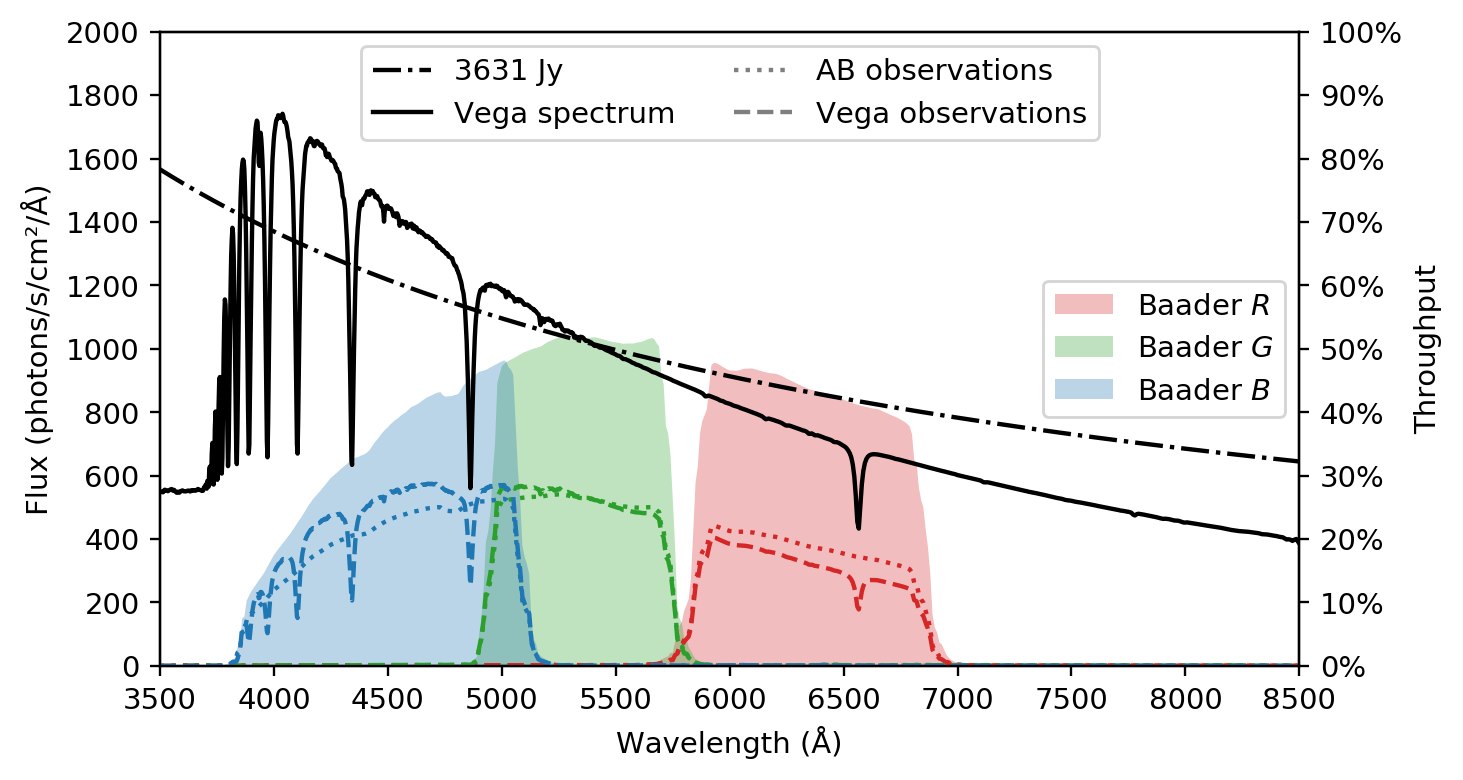
\includegraphics[width=\textwidth]{images/throughput/synphot_RGB.png}
        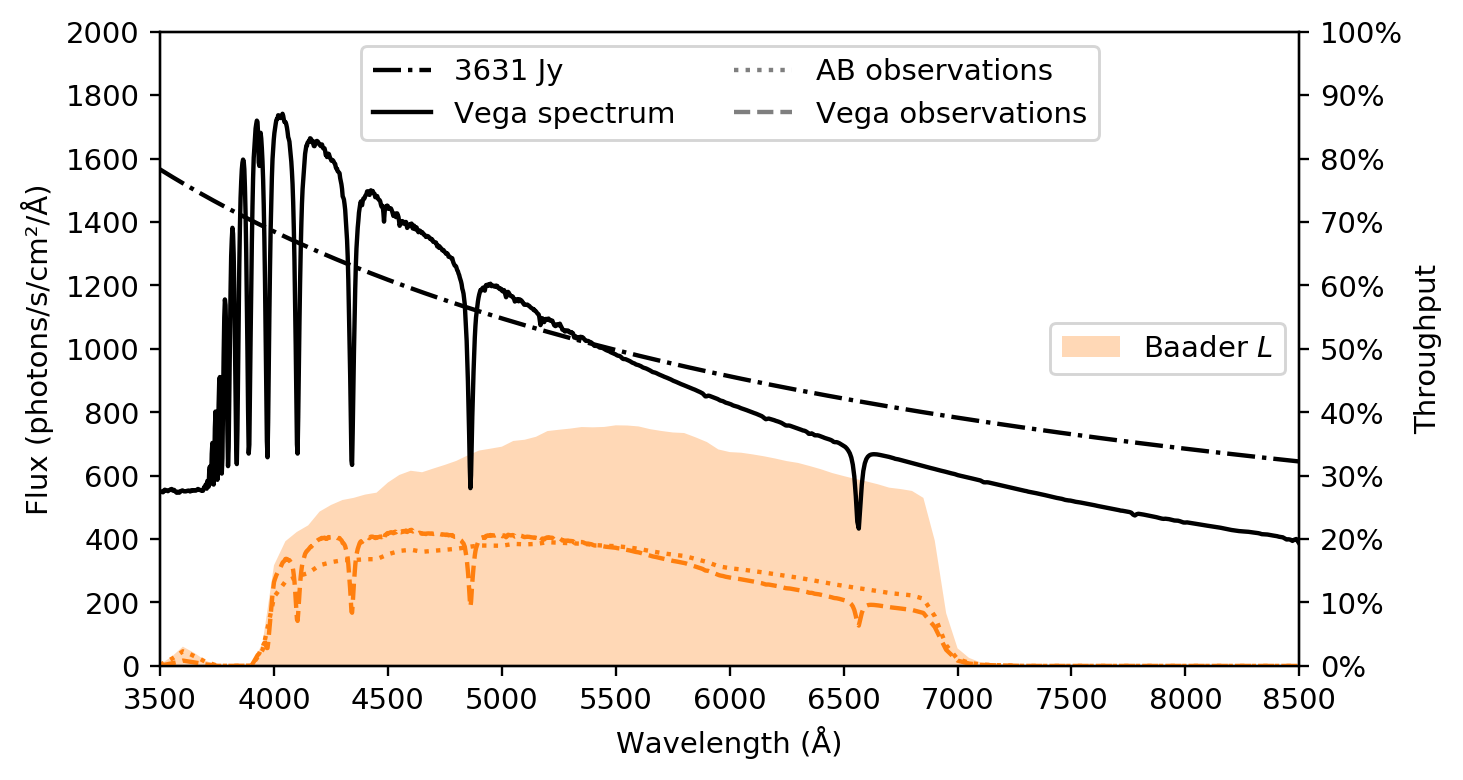
\includegraphics[width=\textwidth]{images/throughput/synphot_L.png}
    \end{center}
    \caption[Simulating photometric observations using pysynphot]{
        Simulating GOTO observations using pysynphot. The filled coloured areas show the theoretical throughputs from \aref{fig:throughput} for the \textit{RGB} filters in the upper plot and the \textit{L} filter in the lower plot. The coloured dotted lines show the throughputs multiplied by a flat \SI{3631}{\jansky} spectrum (dot-dashed black line), while the coloured dashed lines show the throughputs multiplied with the model Vega spectrum (solid black line).
    }\label{fig:pysynphot}
\end{figure}

\clearpage

\end{colsection}

% ~~~~~~~~~~~~~~~~~~~~

\newpage
\subsection{Limiting magnitude}
\label{sec:lim_mag}
\begin{colsection}

Using the CCD parameters determined in \aref{sec:detectors}, the throughput model created in \aref{sec:throughput} and the zeropoints calculated in \aref{sec:model_zeropoints}, a complete photometric model of the GOTO telescopes can be created. One use of this is to predict the system limiting magnitude for a target signal-to-noise ratio.

% ---------
\subsubsection{Signal-to-noise}

The common sources of noise in CCDs are discussed in \aref{sec:noise}. Discounting the bias level and fixed-pattern noise, both properties of the detector that are easy to remove, the major sources of noise in an astronomical image will be the dark current and read-out noise as well as the shot noise from the target and the sky background. Accounting for these the total noise in the image is given by
%
\begin{equation}
    \sigma_\text{Total} = \sqrt{N + N_\text{sky} + D + R^2},
    \label{eq:total_noise}
\end{equation}
%
where $N$ is the electron signal from the source object, $N_\text{sky}$ is the background signal from the sky, $D$ is the dark current and $R$ is the read-out noise. Noise is usually quantified as a fraction of the target signal $N$, known as the signal-to-noise ratio \glsadd{snr}:
%
\begin{equation}
    \text{SNR} = \frac{N}{\sigma_\text{Total}} = \frac{N}{\sqrt{N + N_\text{sky} + D + R^2}}.
    \label{eq:snr}
\end{equation}
%
To be confident of the detection of an astronomical source a signal-to-noise ratio of 5 or more is required, also known as a $5\sigma$ detection (as the signal will be more than 5 times the noise).

\newpage

% ---------
\subsubsection{Sky background noise}

\begin{figure}[t]
    \begin{center}
        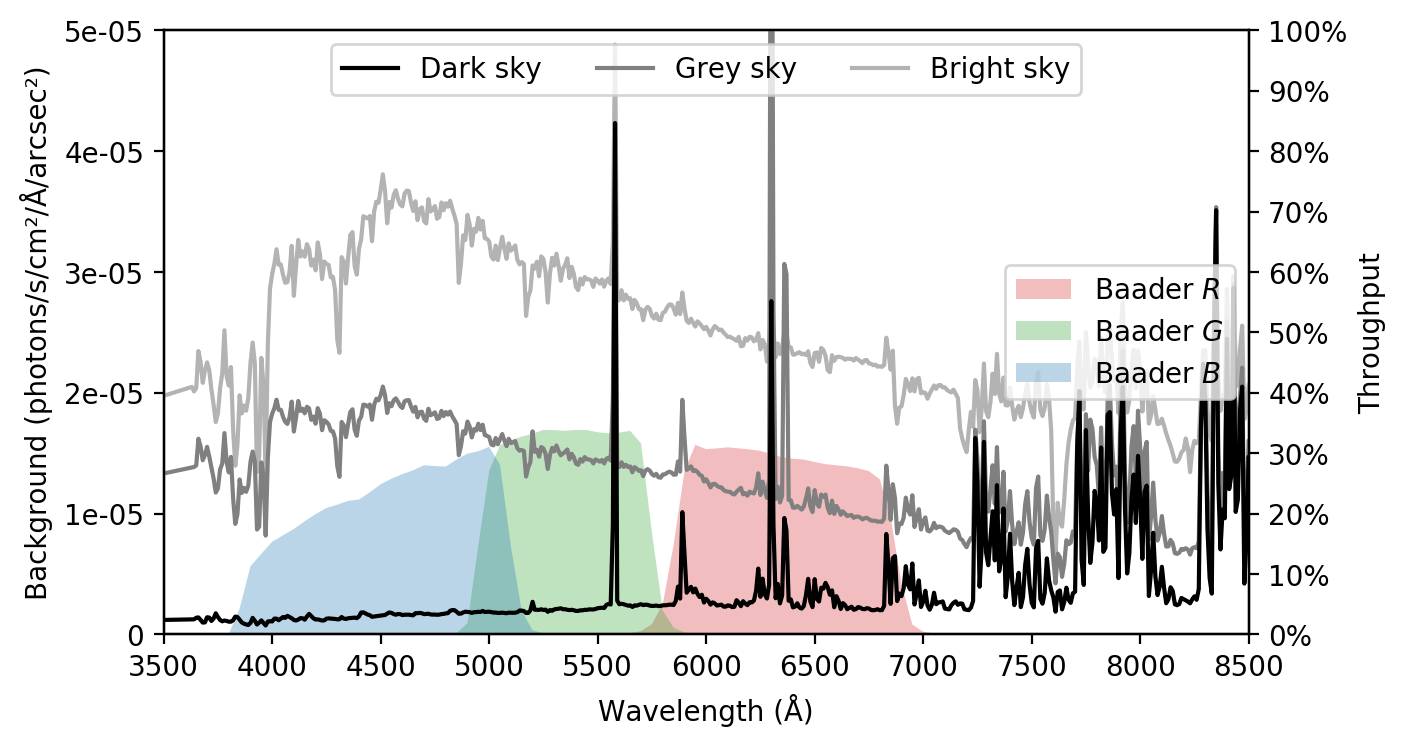
\includegraphics[width=\textwidth]{images/throughput/background.png}
    \end{center}
    \caption[Simulating sky background observations]{
        Simulating sky background observations using pysynphot.
    }\label{fig:background}
\end{figure}

The one value in \aref{eq:snr} that has not yet been considered is the sky background noise, $N_\text{sky}$. The brightness of the sky will change most noticeably as a function of the Moon phase, with a full Moon creating a background noise several magnitudes brighter than during a new Moon or when the Moon is below the horizon. In order to model the background, sky spectra were taken from \citet{sky_background}, which were obtained from 6 years of VLT observations using the FORS1 instrument\footnote{Spectra available at \href{http://www.eso.org/~fpatat/science/skybright}{\texttt{http://www.eso.org/\raisebox{0.5ex}{\texttildelow}fpatat/science/skybright}}}. Three sample spectra were selected to give a range of background signals: a ``Dark'' spectrum taken when the Moon was new and below the horizon, a ``Grey'' spectrum taken when the Moon was 60\% illuminated, and a ``Bright'' spectrum taken when the Moon was full. These spectra are shown in \aref{fig:background}.

In order to determine the sky background noise in the GOTO filters the same method using pysynphot can be used as in \aref{sec:model_zeropoints}. The spectra were again multiplied by the throughput curve for each filter from \aref{sec:total_throughput}, and multiplied by the collecting area of the telescope in order to get an predicted signal in electrons per second. These were converted into instrumental magnitudes using \aref{eq:ins_mag} and then into calibrated magnitudes using \aref{eq:zp} and the AB zeropoints given in \aref{tab:pysynphot_zeropoints}. The resulting signals are given in \aref{tab:pysynphot_background}. Note that the values are given per square arcsecond; when calculating the sky background flux the signal must be multiplied by the squared plate scale of the camera to get the signal per pixel (the plate scale of the GOTO CCDs is 1.24 arcseconds/pixel).

\begin{table}[t]
    \begin{center}
        \begin{tabular}{c|ccc|ccc} %chktex 44
                   & \multicolumn{6}{c}{Thoretical sky signal} \\
            Filter &
            \multicolumn{3}{c|}{(\elec/s/arcsec$^2$)} &
            \multicolumn{3}{c}{(mag/s/arcsec$^2$)} \\
                   & Dark & Grey & Bright & Dark & Grey & Bright \\
            \midrule
            Baader \textit{L} & 2.58 & 14.27 & 27.13 & 21.44 & 19.58 & 18.88 \\
            Baader \textit{R} & 1.18 &  4.37 &  8.20 & 20.99 & 19.58 & 18.89 \\
            Baader \textit{G} & 0.81 &  4.56 &  8.99 & 21.45 & 19.57 & 18.83 \\
            Baader \textit{B} & 0.52 &  5.74 & 10.65 & 22.20 & 19.60 & 18.93 \\
        \end{tabular}
    \end{center}
    \caption[Sky background signals calculated using pysynphot]{
        Sky background signals calculated using pysynphot for different Moon phases, in AB magnitudes.
    }\label{tab:pysynphot_background}
\end{table}

% ---------
\subsubsection{Calculating limiting magnitudes}

The limiting magnitude of a telescope is defined as the signal which would be required to obtain a particular SNR, typically $5\sigma$. \aref{eq:snr} can be rearranged into a quadratic formula
%
\begin{equation}
    N_\text{lim}^2 - \text{SNR}^2 N_\text{lim} + \text{SNR}^2 (N_\text{sky} + D + R^2) = 0,
    \label{eq:snr2}
\end{equation}
%
and this can be solved to find $N_\text{lim}$.

It is important to remember that $N_\text{lim}$, $N_\text{sky}$ and $D$ are in electrons per second per pixel while $R$ is just in electrons per pixel. Each therefore needs to be multiplied by the number of pixels the source is spread across, which will be the determined by the the size of the seeing disk. A given seeing $s$ in arcseconds is defined as the \glsfirst{fwhm} of the seeing disk in the image, which using a Gaussian profile is given by $ 2\sqrt{2 \ln 2}~\sigma$. Taking the $3\sigma$ radius the number of pixels the source will be spread across is
%
\begin{equation}
    n = \pi {\left( \frac{3\sigma}{p} \right) }^2
      = \pi {\left( \frac{3s}{2\sqrt{2 \ln 2}~p} \right) }^2,
    \label{eq:seeing2}
\end{equation}
%
where $p$ is the plate scale in arcseconds/pixel.

Finally, the limiting magnitude in each filter can be calculated for a range of exposure times. These are plotted in \aref{fig:lim_mags} for dark and bright skies, for each GOTO filter and camera. Note that it is almost impossible to distinguish between the curves for each camera, as the differences between their dark and read out noise values are very small. The limiting magnitudes for a \SI{60}{\second} image, the typical exposure time for GOTO observations, are given in \aref{tab:lim_mags}.

\begin{figure}[t]
    \begin{center}
        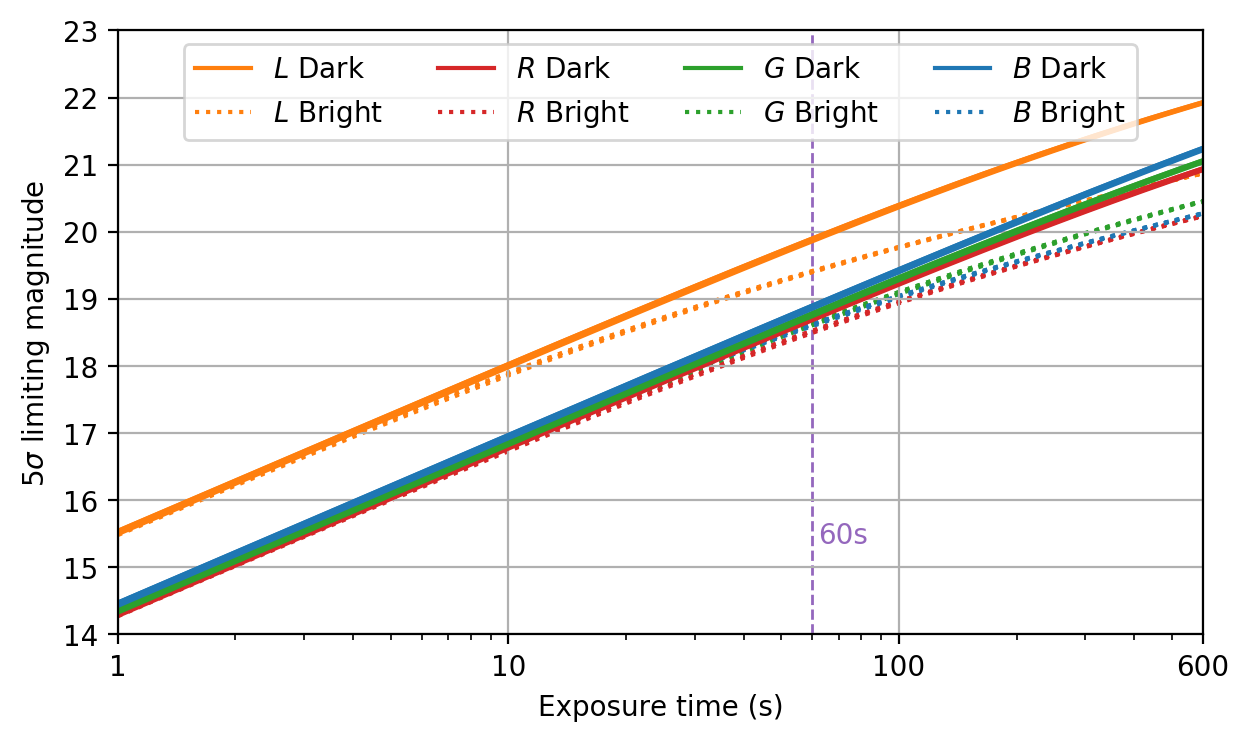
\includegraphics[width=\textwidth]{images/throughput/limiting_mag.png}
    \end{center}
    \caption[$5\sigma$ limiting magnitudes for GOTO]{
        $5\sigma$ limiting magnitudes for GOTO plotted as a function of exposure time, assuming an airmass of 1 and seeing of 1.5''. Solid lines give the limiting magnitude during dark time, dotted lines during bright time. The vertical line marks \SI{60}{\second}, the typical GOTO exposure time.
    }\label{fig:lim_mags}
\end{figure}

\begin{table}[t]
    \begin{center}
        \begin{tabular}{c|ccc} %chktex 44
                   & \multicolumn{3}{c}{Limiting magnitude} \\
            Filter & \multicolumn{3}{c}{(mag)} \\
                   & Dark & Grey & Bright \\
            \midrule
            Baader \textit{L} & 19.76 & 19.53 & 19.35 \\
            Baader \textit{R} & 18.51 & 18.43 & 18.35 \\
            Baader \textit{G} & 18.56 & 18.46 & 18.37 \\
            Baader \textit{B} & 18.85 & 18.72 & 18.62 \\
        \end{tabular}
    \end{center}
    \caption[$5\sigma$ limiting magnitudes for a \SI{60}{\second} exposure]{
        $5\sigma$ limiting magnitudes for a \SI{60}{\second} exposure.
    }\label{tab:lim_mags}
\end{table}

\end{colsection}

% ~~~~~~~~~~~~~~~~~~~~
\newpage
\subsection{Comparison to on-sky observations}
\label{sec:onsky_comparison}
\begin{colsection}

The GOTO prototype finally reached a stable 4-UT configuration in February 2019 (see \aref{sec:timeline}). In order to determine if it was performing to expectations the theoretical zeropoints calculated in \aref{sec:model_zeropoints} and limiting magnitudes calculated in \aref{sec:lim_mag} can be compared to those found from on-sky observations. Since GOTO is a wide-field survey instrument there was no need to observe a particular standard star or field --- each frame contains thousands of sources that can be matched to a photometric catalogue. A set of sample observations were used: three \SI{60}{\second} exposures in each of the four filters (so 12 in total) of the Virgo Cluster, taken on the 16th of March 2019. These observations were taken during dark time when the field was at a high altitude (airmass 1.08).

Each image was processed using the standard GOTOphoto pipeline described in \aref{sec:gotophoto}, which corrected the frames for bias, dark and flat frames and extracted sky-subtracted source counts using Source Extractor \citep{SE}. These counts were converted into instrumental magnitudes using \aref{eq:ins_mag}, with $t=\SI{60}{\second}$ and using the gain values for each camera calculated in \aref{sec:ptc}. As GOTO uses the non-standard Baader filters (see \aref{sec:filters}) there are no catalogue magnitudes to compare to. The GOTO pipeline instead makes do with the best available catalogues: the Pan-STARRS PS1 catalogue \citep{Pan-STARRS} and APASS, the AAVSO Photometric All-Sky Survey \citep{APASS}. The \textit{L} and \textit{G} Baader filters are matched to Pan-STARRS \textit{g}, \textit{R} to Pan-STARRS \textit{r} and \textit{B} to APASS \textit{B}.

\newpage

\begin{figure}[t]
    \begin{center}
        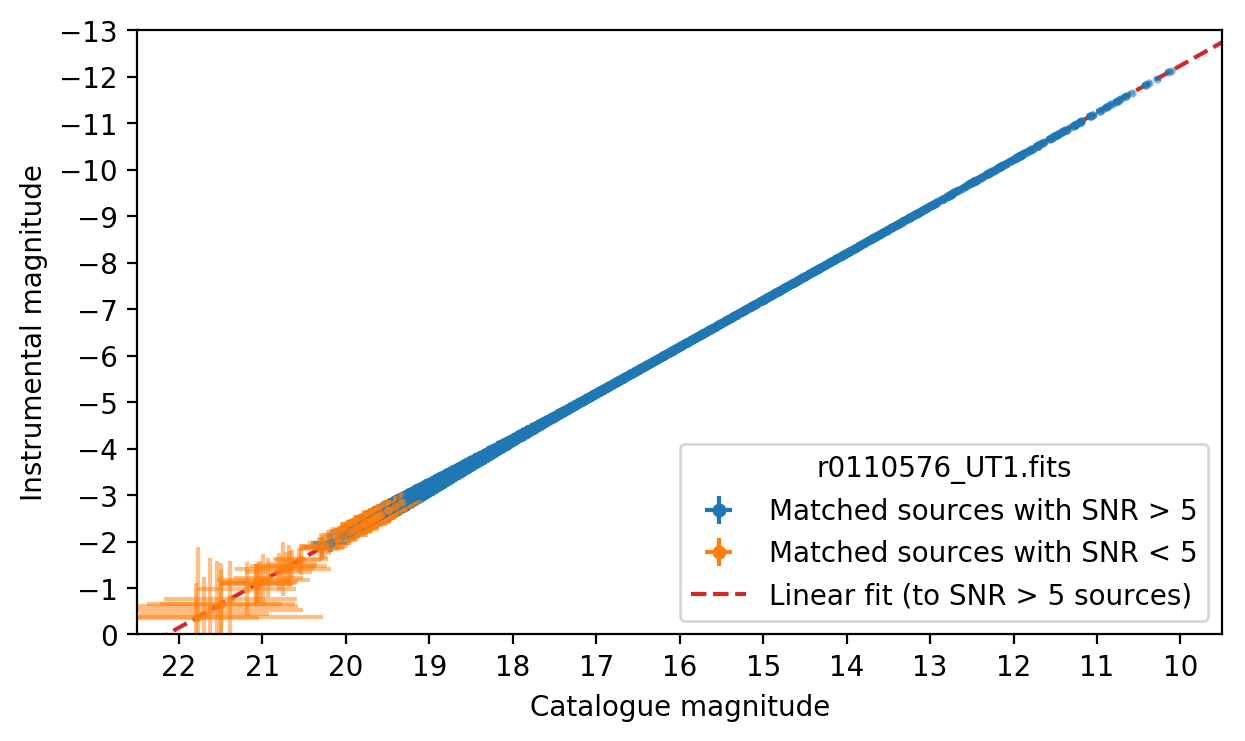
\includegraphics[width=\textwidth]{images/throughput/zeropoint_real.png}
    \end{center}
    \caption[Finding the observed zeropoint from a GOTO image]{
        Finding the observed zeropoint from a GOTO image.
    }\label{fig:zeropoint}
\end{figure}

In order to find the zeropoint for each image a linear function was fitted to the measured instrumental magnitudes of each source as a function of the catalogue magnitude of the star it was matched against, with the $y$-intercept being equal to the zeropoint for that image. This is shown in \aref{fig:zeropoint} for one of the \textit{L}-band images. To exclude faint sources with large errors, only sources with a signal-to-noise ratio of 5$\sigma$ or above were included in the fit. This was repeated for every image, and the zeropoints for each are given in \aref{tab:zps_lms}.

The theoretical zeropoints found in \aref{sec:model_zeropoints} were calculated for zero-magnitude stars above the atmosphere, i.e.\ not including the effects of atmospheric extinction described in \aref{sec:atmosphere}. Obviously the real zeropoints measured from GOTO images will include this effect, and so in order to compare the theoretical values to the observed zeropoints the extinction coefficients from \aref{tab:throughput_extinction} were subtracted (multiplied by 1.08, the airmass of the source at the time it was observed) from the theoretical values. This was done for each filter using the AB magnitudes from \aref{tab:pysynphot_zeropoints}, and the new theoretical zeropoints are given in \aref{tab:zps_comparison} along with the best observed zeropoint from each set of three images.

To measure the limiting magnitude from each image, the catalogue magnitude of each source was compared to the ratio of the source counts to the noise measured by Source Extractor, plotted in \aref{fig:lim_mag}. Sources with a signal-to-noise ratio between 4.5 and 5.5 were plotted on a histogram with bins of 0.1 mag, and the $5\sigma$ limiting magnitude was taken as the bin containing the most sources. The best limiting magnitudes from each set of three are given in \aref{tab:lms_comparison}, along with the theoretical dark-time limiting magnitudes from \aref{tab:lim_mags}.

\begin{figure}[t]
    \begin{center}
        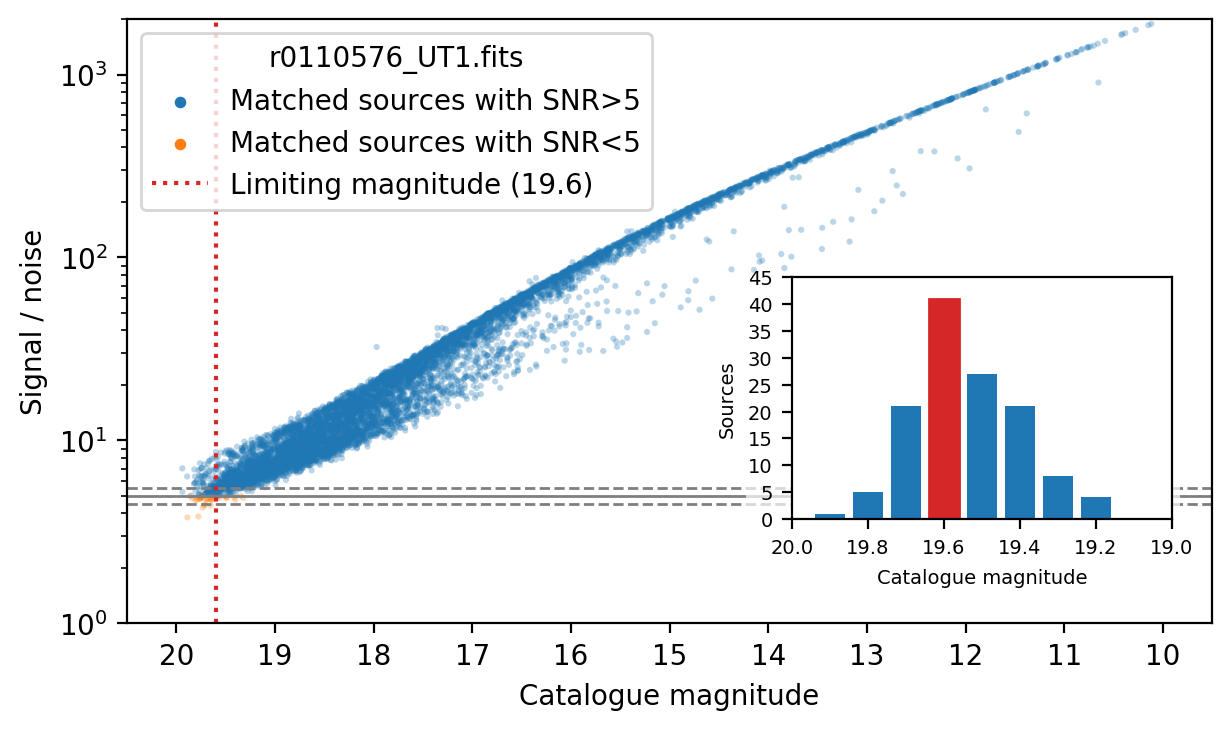
\includegraphics[width=\textwidth]{images/throughput/limiting_mag_real.png}
    \end{center}
    \caption[Finding the limiting magnitude from a GOTO image]{
        Finding the limiting magnitude from a GOTO image. The catalogue magnitude of sources with SNR of between 4.5 and 5.5 (shown by the \textcolorbf{Gray}{grey} horizontal lines) are plotted on a histogram with bins of 0.1 mag (inset), the limiting magnitude is the magnitude of the bin with the highest number of sources (highlighted in \textcolorbf{Red}{red}).
    }\label{fig:lim_mag}
\end{figure}

\newpage

\begin{table}[p]
    \begin{center}
        \begin{tabular}{cc|cc|cc|cc|cc} %chktex 44
             & &
            \multicolumn{2}{c|}{UT1} &
            \multicolumn{2}{c|}{UT2} &
            \multicolumn{2}{c|}{UT3} &
            \multicolumn{2}{c}{UT4}
            \\
             & &
            \multicolumn{2}{c|}{{\footnotesize(ML6094917)}} &
            \multicolumn{2}{c|}{{\footnotesize(ML0010316)}} &
            \multicolumn{2}{c|}{{\footnotesize(ML0420516)}} &
            \multicolumn{2}{c}{{\footnotesize(ML5644917)}}
            \\
            \multicolumn{2}{c|}{Filter} &
            ZP & LM & ZP & LM & ZP & LM & ZP & LM \\
            \midrule
            \textit{L} & 1 &
            22.32 & 19.6 &
            22.31 & 19.6 &
            22.40 & 19.6 &
            22.32 & 19.6
            \\
            & 2 &
            22.26 & 19.6 &
            22.27 & 19.5 &
            22.44 & 19.7 &
            22.37 & 19.6
            \\
            & 3 &
            22.39 & 19.6 &
            22.42 & 19.4 &
            22.45 & 19.6 &
            22.40 & 19.7
            \\
            \midrule
            \textit{R} & 1 &
            20.83 & 18.3 &
            21.05 & 18.2 &
            21.10 & 18.4 &
            21.05 & 18.0
            \\
            & 2 &
            20.84 & 18.2 &
            21.11 & 18.4 &
            21.13 & 18.2 &
            21.06 & 18.0
            \\
            & 3 &
            20.91 & 18.3 &
            21.01 & 18.2 &
            21.04 & 18.4 &
            20.94 & 18.2
            \\
            \midrule
            \textit{G} & 1 &
            21.20 & 18.7 &
            21.39 & 18.5 &
            21.40 & 18.6 &
            21.27 & 18.3
            \\
            & 2 &
            21.16 & 18.6 &
            21.43 & 18.6 &
            21.46 & 18.6 &
            21.36 & 18.4
            \\
            & 3 &
            21.26 & 18.7 &
            21.44 & 18.7 &
            21.45 & 18.8 &
            21.32 & 18.5
            \\
            \midrule
            \textit{B} & 1 &
            21.22 & 18.9 &
            21.35 & 19.0 &
            21.43 & 19.1 &
            21.27 & 18.9
            \\
            & 2 &
            21.22 & 19.0 &
            21.32 & 18.8 &
            21.44 & 19.1 &
            21.22 & 18.9
            \\
            & 3 &
            21.20 & 19.1 &
            21.35 & 18.9 &
            21.44 & 19.1 &
            21.26 & 18.8
            \\
        \end{tabular}
    \end{center}
    \caption[Observed zeropoints and limiting magnitudes]{
        Observed zeropoints (ZP) \glsadd{zp} and limiting magnitudes (LM) \glsadd{lm} from three \SI{60}{\second} exposures taken in each filter. The camera serial numbers can be matched to \aref{tab:cameras}.
    }\label{tab:zps_lms}
\end{table}

\begin{table}[p]
    \begin{center}
        \begin{tabular}{c|c|cccc|cccc} %chktex 44
             &
            Theoretical &
            \multicolumn{4}{c|}{Best observed zeropoint} &
            \multicolumn{4}{c}{Difference (obs-theory)}
            \\
            Filter & zeropoint & UT1 & UT2 & UT3 & UT4 & UT1 & UT2 & UT3 & UT4 \\
            \midrule
            \textit{L} & 22.45 & 22.39 & 22.42 & 22.45 & 22.40 & -0.06 & -0.03 &  0.00 & -0.05 \\
            \textit{R} & 21.17 & 20.91 & 21.11 & 21.13 & 21.06 & -0.26 & -0.06 & -0.04 & -0.11 \\
            \textit{G} & 21.21 & 21.26 & 21.44 & 21.46 & 21.36 & +0.05 & +0.23 & +0.25 & +0.15 \\
            \textit{B} & 21.47 & 21.22 & 21.35 & 21.44 & 21.27 & -0.25 & -0.12 & -0.03 & -0.20 \\
        \end{tabular}
    \end{center}
    \caption[Comparison between theoretical and observed zeropoints]{
        Comparison between the theoretical zeropoints (accounting for extinction) and the best observed zeropoints.
    }\label{tab:zps_comparison}
\end{table}

\begin{table}[p]
    \begin{center}
        \begin{tabular}{c|c|>{\centering\arraybackslash}p{1.2cm}>{\centering\arraybackslash}p{1.2cm}>{\centering\arraybackslash}p{1.2cm}>{\centering\arraybackslash}p{1.2cm}} %chktex 44
             &
            Theoretical &
            \multicolumn{4}{c}{Best observed limiting magnitude}
            \\
            Filter & limiting magnitude & UT1 & UT2 & UT3 & UT4 \\
            \midrule
            \textit{L} & 19.76 & 19.6 & 19.6 & 19.7 & 19.6 \\
            \textit{R} & 18.51 & 18.3 & 18.4 & 18.4 & 18.2 \\
            \textit{G} & 18.56 & 18.7 & 18.7 & 18.8 & 18.5 \\
            \textit{B} & 18.85 & 19.1 & 19.0 & 19.1 & 18.9 \\
        \end{tabular}
    \end{center}
    \caption[Comparison between theoretical and observed limiting magnitudes]{
        Comparison between the theoretical limiting magnitudes (for dark time) and the best observed limiting magnitudes.
    }\label{tab:lms_comparison}
\end{table}

\clearpage

In most cases the observed zeropoints and limiting magnitudes are very close to the theoretical values. Further images taken over more nights are needed to make any firm conclusions, but a few trends are clear. UT3 consistently has better zeropoints than the other unit telescopes, which might be because its mirrors were re-aluminised and returned to La Palma only a month before the images were taken (see \aref{sec:timeline}). Therefore the difference in the observed and theoretical zeropoints may be due to a lower mirror reflectivity than assumed in throughput model in \aref{sec:optics} (e.g.\ due to dust build up on the mirrors). It also seems that the throughput in the \textit{G} band has been underestimated, as the observations taken in the \textit{G} filter consistently have higher zeropoints and better limiting magnitudes than predicted. This may be due to the bandwidth being wider than modelled, as any other change in throughput would also affect the other filters.

\end{colsection}

% ~~~~~~~~~~~~~~~~~~~~

\end{colsection}

% ########################################
